\documentclass[final]{elsarticle}
%\usepackage[pdftex,breaklinks,linktocpage,pagebackref,hyperindex,hyperfigures]
\usepackage{hyperref}
\usepackage[utf8]{inputenc}
\usepackage{amsmath}
\usepackage{amsthm}
\usepackage{amssymb}
\usepackage[tmargin=1in,bmargin=1in,lmargin=1in,rmargin=1in]{geometry}
\usepackage{subfigure}
\usepackage{graphicx}
\usepackage{latexsym}
\usepackage{pdfsync}
\usepackage[boxed]{algorithm}
\usepackage{algpseudocode}
\usepackage{algorithm}
%\usepackage{algorithmic}
\usepackage{multirow}
\usepackage{rotating}
\usepackage{color}
\usepackage{caption}
\usepackage{url}

\hypersetup{
    colorlinks=true,      		% false: boxed links; true: colored links
    linkcolor=blue,       		% color of internal links
    citecolor=blue,       		% color of links to bibliography
    filecolor=black,      		% color of file links
    urlcolor=red,       		% color of external links
    bookmarks=false,
    pdffitwindow=true,
    pdfpagelayout=SinglePage
}

% defining some new commands
\newcommand{\etal}{\textit{et al.\ }}
\newcommand{\mbf}[1]{\mathbf{#1}}
\newcommand{\comment}[1]{\textcolor{red}{#1}}
\newcommand{\tensor}[1]{\underline{\underline{\boldsymbol{#1}}}}
\newcommand{\be}{\begin{equation}}
\newcommand{\ee}{\end{equation}}
\newcommand{\ben}{\begin{equation*}}
\newcommand{\een}{\end{equation*}}
\newcommand{\bea}{\begin{eqnarray}}
\newcommand{\eea}{\end{eqnarray}}
\newcommand{\bean}{\begin{eqnarray*}}
\newcommand{\eean}{\end{eqnarray*}}
\newcommand{\pd}[2]{\frac{\partial #1}{\partial #2}}
\newcommand{\pdn}[3]{\frac{\partial^#1 #2}{\partial #3^#1}}
\newcommand{\noi}{\noindent}
\newcommand{\ind}{\indent}
\newcommand{\divg}[1]{\nabla \cdot \left(#1\right)}
\newcommand{\ddivg}[1]{\nabla \cdot #1}
\newcommand{\non}{\nonumber}
\newcommand{\fcite}[1]{(\textcolor{blue}{cite: #1})}
\newtheorem{property}{Property}

\begin{document}

\title{Tree-based Adaptive Level-set Methods on Highly Parallel Machines}

\cortext[cor]{Corresponding author: m.mirzadeh@engineering.ucsb.edu}
\address[MECHE]{Department of Mechanical Engineering, University of California, Santa Barbara, CA 93106-5070, United States.}
\address[CS]{Department of Computer Science, University of California, Santa Barbara, CA 93106-5110, United States.}
\address[UBONN]{Institute for Numerical Simulation, University of Bonn, Bonn 53115, Germany.}

\author[MECHE]{Mohammad Mirzadeh\corref{cor}} \author[MECHE]{Arthur Guittet} \author[UBONN] {Carsten Burstedde} \author[MECHE,CS]{Fr\'ed\'eric Gibou}

%!TEX root = draft.tex
\begin{abstract}
In this article we present scalable parallel algorithms for the advection and reinitialization of level-set functions on adaptive Quadtree and Octree grids. Our algorithms are based on domain decomposition technique and implemented using \texttt{MPI} and the open-source \texttt{p4est} library. An important contribution of the paper is a parallel semi-Lagrangian method which, similar to its serial implementation, is free of any time-step restrictions. This is achieved by introducing a scalable global interpolation scheme on adaptive Quadtree and Octree grids. Moreover, we present a simple parallel reinitialization scheme using the pseudo-time transient formulation. Both parallel algorithms scale nicely on the Stampede supercomputer where we are limited to 4096 cores at most. Finally a relevant application of the algorithms is presented in modeling the crystallization phenomena by solving a Stefan problem, illustrating a level of detailed calculation that would be impossible on uniform grids. We believe that the algorithms presented in this article will be of interest and useful to researchers working with the level-set framework and modeling multi-scale physics in general.
\end{abstract}
\begin{keyword}
Quadtree/Octree Grids \sep Parallel Computing \sep Space Filling Curves \sep Semi-Lagrangian Method \sep Level-set Method
\end{keyword}
\maketitle

%!TEX root = draft.tex
\section{Introduction}\label{sec:introduction}
The level-set method, originally proposed by Sethian and Osher \cite{Osher;Sethian:88:Fronts-Propagating-w}, is a popular and powerful framework for tracking arbitrary interfaces that undergo complicated topological changes. As a result, the level-set method has wide range of application such as multiphase flows, moving boundary problems, image segmentation, and computer graphics \cite{Osher;Fedkiw:01:Level-Set-Methods:-A,Sethian:99:Level-set-methods-an}. An important feature which makes this method powerful and easy to use is that the location of interface is defined implicitly on an underlying grid. This convenience, however, comes at a price. First, compared to an explicit method, e.g. front tracking \cite{Juric:96:A-Front-Tracking-Met, Tryggvason;Bunner;Esmaeeli;etal:01:A-Front-Tracking-Met}, the level-set method is typically less accurate and mass conservation could be a problem; although progress has been made in resolving this issue \cite{Enright;Fedkiw;Ferziger;etal:02:A-Hybrid-Particle-Le}. Second, the level-set function has to be defined in a higher dimensional space compared to the interface. If only the location of the interface is needed, the added dimension greatly increases the overall computational cost. One way to avoid this problem is by computing the level-set only close to the interface, e.g. as in the narrow-band level-set method \cite{Adalsteinsson;Sethian:95:A-Fast-Level-Set-Met} or, more recently, by using a hash table to restrict both computation and storage requirements \cite{Brun;Guittet;Gibou:12:A-local-level-set-me}.

Another approach that can address both problems is the use of local grid refinement. In \cite{Strain:99:Tree-Methods-for-Mov} the idea of using tree-based grids for level-set calculations was first introduced and later extended in \cite{Losasso;Gibou;Fedkiw:04:Simulating-Water-and} for graphics application. More recently, authors in \cite{Min;Gibou:07:A-second-order-accur} proposed second-order accurate level-set methods on Quadtree (two spatial dimensions) and Octree (three spatial dimensions) grids. The use of tree-based adaptive grids in the context of the level-set method is quite advantageous because: 1) It gives fine-grain control over errors, which typically occur close to the interface and 2) It can effectively reduce the dimensionality of the problem by focusing most of the grid cells close to the interface. Fortunately, constructing the tree is quite simple in the presence of an interface that naturally defines an ideal metric for refinement. Although the use of adaptive grids can dramatically reduce the computational cost, performing high-resolution three dimensional calculations of complex interfacial problems, e.g. crystal growth in binary alloys \cite{Theillard;Gibou;Pollock:14:A-Sharp-Computationa}, could take a very long time in serial. In this paper we extend these algorithms by proposing parallel algorithms for distributed memory machines using a domain decomposition technique.

One of the main challenges in parallelizing level-set algorithms on adaptive grids is handling the grid itself. One option is to replicate the entire grid on each processor and use off-the-shelf graph partitioners, e.g. ParMetis \cite{Karypis;Kumar:98:A-parallel-algorithm} or Zoltan \cite{Boman;Catalyurek;Chevalier;etal:12:The-Zoltan-and-Isorr}, for load balancing and domain decomposition. For instance, this was the approach originally taken by the \texttt{deal.II} library \cite{Bangerth;Hartmann;Kanschat:07:deal.II----a-General}. This approach, however, is only scalable to a few hundred processors at best and is limited by the size of the grid itself. Moreover, the use of a general-purpose graph partitioner adds extra overhead that can limit the overall scalability even further. Interestingly, tree-based grids have nice spatial ordering that naturally leads to the concept of space-filling curves (SFCs) which can be efficiently exploited for parallel load balancing \cite{Aluru;Sevilgen:97:Parallel-domain-deco,Campbell;Devine;Flaherty;etal:03:Dynamic-octree-load-}.

The idea of using SFCs for parallel partitioning of Quad-/Octrees is not new in itself and has been tried by many researchers. For instance, \texttt{Octor} \cite{Tu;OHallaron;Ghattas:05:Scalable-parallel-oc} uses a Morton curve (also known as Z-curve) for traversing the leaves of an Octree for indexing and load balancing and has been scaled up to 62,000 cores \cite{Burstedde;Ghattas;Gurnis;etal:08:Scalable-adaptive-ma}. \texttt{Dendro} \cite{Sampath;Adavani;Sundar;etal:08:Dendro:-parallel-alg} is another example of an octree code in which similar ideas are used for parallel partitioning and development of a parallel geometric multigrid that has been scaled up to about 32,000 cores \cite{Sampath;Biros:10:A-parallel-geometric}. More recently, authors in \cite{Burstedde;Wilcox;Ghattas:11:p4est:-Scalable-Algo} extended these ideas to a collection, or a ``forest'', of Octrees that are connected through a common, potentially unstructured, hexahedral grid. This forest is then partitioned in parallel using a global Morton curve. The implementation of these algorithms, which were shown to scale to more than 200,000 processors, is publicly available through a simple API provided by the \texttt{p4est} library \cite{p4est-github}. In fact the algorithms presented in this paper are directly implemented on top of the \texttt{p4est} library and we do not discuss any algorithm that is already covered in \cite{Burstedde;Wilcox;Ghattas:11:p4est:-Scalable-Algo}. We also make use of the popular \texttt{PETSc} \cite{Balay;Abhyankar;Adams;etal:14:PETSc-Web-page} library for linear algebra and its parallel primitives, such as parallel ghosted vector and scatter/gather operations, which simplifies the implementation. 

Parallel level-set algorithms can be categorized in two groups: 1) Parallel advection algorithms and 2) Parallel reinitialization algorithms. Eulerian advection schemes can easily be parallelized but unfortunately are limited by the CFL condition which could be very restrictive for adaptive grids. Semi-Lagrangian methods combine the unconditional stability of Lagrangian methods and the ease of use of Eulerian grids and have been successfully used for advecting the level-set function on tree-based grids in the past \cite{Min;Gibou:07:A-second-order-accur}. However, parallelizing the semi-Lagrangian algorithm in a domain decomposition context is not an easy task. The reason for this is twofold. First, depending on the CFL number, the departure points may end up outside the ghost region and in remote processors that are potentially far away. This requires a very dynamic and nonuniform communication pattern which is complicated to implement. For an adaptive grid situation, it is even more complicated due to the asymmetric nature of the communication (c.f. \ref{sec:parallel algorithms}). Second, load balancing could be an issue for large CFL numbers and nonuniform velocity fields due to clustering of departure points and can considerably restrict the scalability of the algorithm. Both of these problems, of course, could be avoided by choosing $\text{CFL} \le 1$ but that would defeat the purpose of using semi-Lagrangian algorithm in the first place. 

Nonetheless, several parallel semi-Lagrangian algorithms have been proposed in the past. A simple domain decomposition technique was used in \cite{Thomas;Cote:95:Massively-parallel-s} where the width of the ghost layer is fixed based on the maximum CFL number to ensure that all the departure points are covered by the ghost layer. At large CFL numbers, this leads to a large volume of communication that can limit the scalability. Nonetheless good scaling was reported for small CFL numbers ($\text{CFL} \le 2$). In \cite{Drake;Foster;Michalakes;etal:95:Design-and-performan} the authors propose a more sophisticated domain decomposition approach which uses a ``dynamic ghost layer''. Here the width of the ghost layer is dynamically determined at runtime based on information from previous time steps. Unfortunately, however, this approach seems to suffer from excessive communication overhead at larger numbers of processors as well \comment{as well ?}. More recently, the authors in \cite{White-III;Dongarra:11:High-performance-hig} used a domain decomposition strategy on a cubed sphere but with a single layer of ghost nodes. Interpolation on remote processors is then handled by sending query points to the corresponding processor and asking for the interpolated result. This approach seems to provide good scalability for transporting a single tracer up to about 1000 cores for $\text{CFL} \sim 10$. At higher CFL numbers the method begins to loose scalability due to an increase in communication volume. Although in this article we are mainly interested in parallel semi-Lagrangian methods, one could resort to finite difference or finite element discretization methods if small CFL numbers are acceptable. Indeed several algorithms of this type have been proposed with applications in modeling dendritic crystal growth \cite{Wang;Chang;Kale;etal:06:Parallelization-of-a}, multiphase flows \cite{Sussman:05:A-parallelized-adapt, Fortmeier;Bucker:11:A-parallel-strategy-, Rodriguez;Sahni;Lahey-Jr;etal:13:A-parallel-adaptive-}, and atomization process \cite{Herrmann:10:A-parallel-Eulerian-}.
%, and image segmentation on GPUs \cite{Lefohn;Cates;Whitaker:03:Interactive-GPU-base,Cates;Lefohn;Whitaker:04:GIST:-an-interactive,Roberts;Packer;Sousa;etal:10:A-work-efficient-GPU}.

In many applications of the level-set method, it is desirable for the level-set function to be a signed distance function, i.e. $|\nabla \phi| = 1$. There are generally two approaches to enforce this property: 1) Solving the pseudo-time transient reinitialization equation \cite{Sussman;Smereka;Osher:94:A-Level-Set-Approach, Osher;Fedkiw:01:Level-Set-Methods:-A}:
\ben
\phi_\tau + S(\phi_0)\left(|\nabla \phi| - 1\right) = 0,
\een
or 2) Solving the Eikonal equation:
\ben
F(x)|\nabla\phi| = 1,
\een 
with constant speed function $F(x) \equiv 1$. The transient reinitialization equation can be solved using explicit finite differences and thus can easily be parallelized in a domain decomposition approach. Moreover, only a few iterations may be needed if the signed-distance property is only required close to the interface \cite{Min;Gibou:07:A-second-order-accur}. This is the approach we have chosen in this paper. However, if the signed-distance property is required in the entire domain solving the Eikonal equation is more computationally efficient. Unfortunately, the most popular algorithm for solving the Eikonal equation, i.e. the Fast Marching Method \cite{Sethian:96:A-Fast-Marching-Leve,Sethian:99:Level-set-methods-an}, is inherently sequential due to causal relationship between grid points and cannot be easily parallelized. The Fast Sweeping Method (FSM) \cite{Zhao:05:A-fast-sweeping-meth} is an alternative method for solving the Eikonal equation iteratively. The FSM can be more computationally efficient for simple choices of speed function, e.g. as in this context, and for simple interfaces. Moreover, FSM has more potential for parallelization compared to the FMM.

One of the earliest attempt in parallelizing the FMM is reported in \cite{Herrmann:03:A-domain-decompositi} where a domain decomposition algorithm was introduced. Unlike the serial FMM, however, parallel FMM potentially requires multiple iterations or ``rollback operations'' to enforce the causality across processors. Similar ideas are described in details in \cite{Tugurlan:08:Fast-marching-method}. It should be noted that the number of iterations needed for the parallel FMM to converge greatly depends on the complexity of the interface and on the parallel partitioning and, in general, fewer iterations are required if the domains are aligned with the normals to the interface. Due to the nature of the Eikonal equation, shared memory machines might be a better environment for parallelization. For instance, in \cite{Breus;Cristiani;Gwosdek;etal:11:An-adaptive-domain-d} the authors use an ``adaptive'' technique where individual threads implicitly define a domain decomposition at runtime. Unfortunately, this approach does not seem to be more effective than a simple static decomposition. In \cite{Zhao:07:Parallel-implementat} a parallel FSM method was presented for the fist time. However, a more scalable FSM was more recently proposed in \cite{Detrixhe;Gibou;Min:13:A-parallel-fast-swee} where the Cuthill-McKee numbering was utilized to expose more parallelism. More recently a two-scale, hybrid FMM-FSM was presented in \cite{Chacon;Vladimirsky:13:A-parallel-Heap-Cell} which, albeit being more complicated to implement, promises even better scalability. Finally, a parallel Fast Iterative Method (FIM) was proposed in \cite{Jeong;Whitaker:08:A-fast-iterative-met}. The FIM is similar to FMM in that it also maintains a list of ``active nodes''. However, unlike FMM, FIM avoids sorting the list and allows for concurrent updating of all nodes in an iterative fashion. \comment{Shouldn't we say that concluding from this analysis, we choose to use iterative reinitialization ?}

The rest of this article is organized as follows: In section \ref{sec:levelset method} we briefly review the sequential algorithms and discretization methods for the level-set equation on adaptive tree-based grids. These ideas are then extended in section \ref{sec:parallel algorithms} to parallel using a domain decomposition method. In section \ref{sec:scaling} we provide several examples that illustrate the scalability of our algorithms. Finally, we close by providing an important application of our algorithms in modeling the solidification process by solving a Stefan problem in \ref{sec:application}.

% %!TEX root = draft.tex
\section{The level-set method}\label{sec:levelset method}
The level-set method, introduced in \cite{Osher;Sethian:88:Fronts-Propagating-w}, is an implicit framework for tracking interfaces that undergo complicated topological changes. In this framework, an interface is represented by the zero contour of a higher dimensional function, e.g.\ a curve in two spatial dimensions can be described as $\Gamma = \{(x,y) | \phi(x,y) = 0\}$, where $\phi(x,y)$ is the level-set function. The evolution of the curve under a velocity field $\underline{\mbf{u}}$ is then obtained by solving the level-set equation:
\be
\phi_t + \underline{\mbf{u}} \cdot \underline{\nabla} \phi = 0.
\label{eq:ls}
\ee
When the velocity field does not depend on the level-set function itself, equation \eqref{eq:ls} can be solved using the semi-Lagrangian method. An important advantage of the semi-Lagrangian method over the regular finite difference method is its unconditional stability, which allows for arbitrarily large time steps. This is particularly important when using adaptive grids, as higher grid resolutions translate into unpractical smaller time steps.

In general, an infinite number of level-set functions can describe the same zero contour and thus an interface. However, it is desirable to chose a function with the signed distance property, i.e.\ $|\underline{\nabla} \phi| = 1$. As detailed in section \ref{sec:introduction}, we solve the pseudo-time transient reinitialization equation \cite{Sussman;Smereka;Osher:94:A-Level-Set-Approach, Osher;Fedkiw:01:Level-Set-Methods:-A} to achieve this property,
\be
\phi_\tau + S(\phi_0)\left(\lvert \underline{\nabla} \phi \rvert - 1\right) = 0,
\label{eq:reinitialization}
\ee
where $\tau$ is a pseudo time step, $\phi_0$ is any level-set function that correctly describes the interface location and $S(\phi_0)$ is an appropriate approximation of the sign function. Here, we do not go into the details of the sequential algorithms for solving equations \eqref{eq:ls} and \eqref{eq:reinitialization}. Instead, we note that the algorithms presented in section \ref{sec:parallel algorithms} are based on the sequential methods presented in \cite{Min;Gibou:07:A-second-order-accur} and refer the interested reader to the aforementioned articles and references therein for more details.
% %!TEX root = draft.tex
\section{Parallel algorithms}\label{sec:parallel algorithms}
\subsection{Grid management}
Adaptive tree-based grids can significantly reduce the computational cost of level-set methods by restricting the fine grid close to the interface where it is most needed \cite{Strain:99:Tree-Methods-for-Mov}. Moreover, adaptive tree-based grids are easy to generate in the presence of a signed-distance level-set function \cite{Min;Gibou:07:A-second-order-accur} and can efficiently be encoded using a tree datastructure \cite{Samet:90:Applications-of-Spat}. To develope scalable parallel algorithms on these grids, it is necessary to parallelize the datastructure and grid manipulations method such as refinement and coarsening of cells as well as provide with a fast method for grid partitioning and load balancing. \texttt{p4est} library \cite{p4est-github} is a collection of such parallel algorithms that has recently emerged and shown to scale up to 200,000 processors \cite{Burstedde;Wilcox;Ghattas:11:p4est:-Scalable-Algo}.

In \texttt{p4est} the adaptive grid is represented as a non-overlapping collection of trees that are rooted in individual cells of a common coarse grid (c.f. figure \ref{fig:p4est_zcurve}). This common coarse grid, which we will refer to as the ``macromesh'', can in general be an unstructured quadrilateral, in two spatial dimensions, or hexahedral mesh, in three spatial dimensions. In this article, however, we shall limit ourselves to simple uniform Cartesian macromeshes. Moreover it is implicitly assumed that the macromesh is small enough that can be entirely replicated on all processors. For instance, in many of the applications that we are interested in this paper the macromesh simply a single cell. \texttt{p4est} allows for arbitrary refinement and coarsening criteria through defining callback functions. In this article the refinement criteria is chosen based on the distance of individual cells to the interface. Specifically a cell $C$ is marked for refinement if:
\be
\min_{\forall v \in V(C)} |\phi| \le \frac{L D}{2}.
\label{eq:refine}
\ee
Conversely an existing cell is marked for coarsening if:
\be
\min_{\forall v \in V(C)} |\phi| > L D.
\label{eq:coarsen}
\ee
Here $V(C)$ denotes the set of all vertices of cell $C$, $L$ denotes the Lipschitz constant of the level-set function, and $D$ denotes the diagonal size of cell $C$. We refer to section 3.2 of \cite{Burstedde;Wilcox;Ghattas:11:p4est:-Scalable-Algo} for details on parallel refinement and coarsening algorithms used in \texttt{p4est}.

Once the gird is adapted to the interface, it must be partitioned to ensure load balancing across processors. This is achieve by constructing a Z-curve that traverses the leaves of all trees in order of tree index (c.f. figure \ref{fig:p4est_zcurve}). A Z-curve is a Space Filling Curve (SFC) with the important property that cells with close Z-indecies are also geometrically close in the physical domain. This is beneficial since it both leads to reduction in MPI communication and improves the cache performance of several algorithms such as interpolation and finite difference calculations. For more details on parallel partitioning in \texttt{p4est} one may refer to section 3.3 of \cite{Burstedde;Wilcox;Ghattas:11:p4est:-Scalable-Algo}.
\begin{figure}[hbtp]
\begin{center}
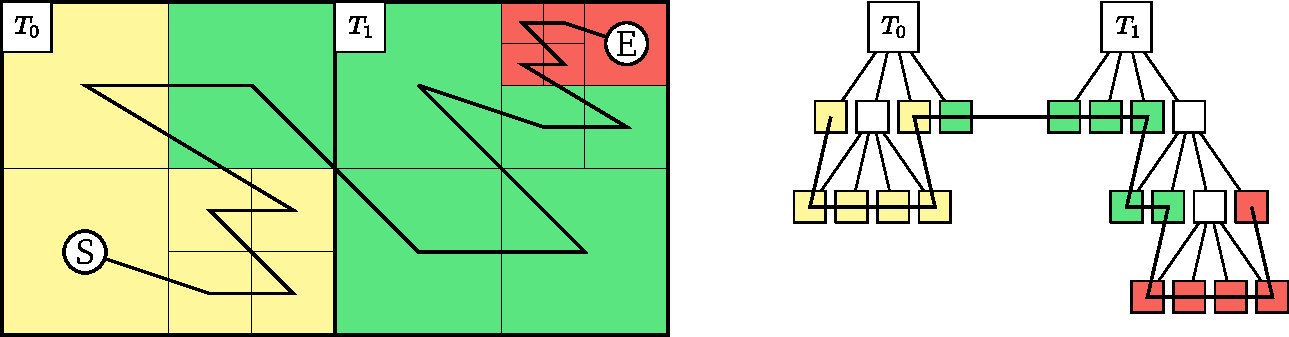
\includegraphics[width = \columnwidth]{figures/p4est_zcurve.pdf}
\caption{Left: A ``forest'' made up of two trees $k_0$ and $k_1$. Parallel partitioning is achieved by first constructing a Z-curve which starts at cell ``S'' and ends at cell ``E''. Next this tree is split up among processors either uniformly or by assigning different weights to cells. Here processors are represented via different colors. Note how use of Z-curve naturally leads to clustering of most cells in each processor domain. Right: Schematic of a tree data structure representing the forest and its partitioning.}
\label{fig:p4est_zcurve}
\end{center}
\end{figure}
Aside from grid manipulation and partitioning, we use two additional features of \texttt{p4est}, namely generation of ghost layer cells and creating a globally unique node indexing. These algorithms are detailed in sections 3.5 and 3.6 of \cite{Burstedde;Wilcox;Ghattas:11:p4est:-Scalable-Algo}. An important feature of our algorithms is that they are designed for non-graded trees. This is important because we can entirely skip tree balancing which was shown to be one of most time consuming parts of grid adaptation in \texttt{p4est} \cite{Burstedde;Wilcox;Ghattas:11:p4est:-Scalable-Algo}.

Finally, in \texttt{p4est} trees are linearized, i.e. only the leaves are explicitly stored. However, all of algorithms considered here require explicit knowledge of the entire tree. As a result we introduce a simple algorithm, called \texttt{Reconstruct}, which recreates a local representation of the entire ``forest'' that is only adapted to local cells and, potentially, the ghost layer. This approach is similar to the ideas introduced in \cite{Bangerth;Burstedde;Heister;etal:11:Algorithms-and-data-} and our tests show that in a typical application they usually amount to less that $1\%$ of the entire runtime. Algorithm \ref{alg:reconstruction} illustrates how this reconstruction is performed. Given a forest and a layer of ghost cells from \texttt{p4est}, the algorithm generates a local representation of forest by recursively refining from the root until reaching the same level and location of all leaves in \texttt{p4est} and \texttt{ghost}. Note that algorithm \ref{alg:reconstruction} does not involve any communication and is load balanced. Figure \ref{fig:reconstruction} illustrates an application of algorithm \ref{alg:reconstruction}. Note how each processor has independently generated a local representation of the forest that is refined to match the same leaves as in the global forest and ghost layer.
% , and has an average runtime complexity of $\mathcal{O}\left((n_l + n_g)\log_{2^d}N\right)$ for well-balanced trees in $d$ dimensions. Here, $n_l$ and $n_g$ are the number of local and ghost cells, respectively, and $N$ is the global number of cells.
\begin{algorithm}[htbp]
\caption{$H \gets \texttt{Reconstruct (}G\texttt{)}$}\label{euclid}
\begin{algorithmic}[1]
\State $H \gets G.\texttt{macromesh()}$
\For {$tr : G.\texttt{local\_trees()}$} \Comment{traverse local cells}
	\For {$q : tr.\texttt{cells()}$}
		\State $H.\texttt{update\_tree(} tr, q \texttt{)}$
	\EndFor
\EndFor

\For {$q : G.\texttt{ghost\_cells()}$} \Comment{traverse ghost cells}
	\State $H.\texttt{update\_tree(} q.\texttt{tree()}, q \texttt{)}$
\EndFor

\State \Return $H$
\\
\Function{$H.\texttt{update\_tree}$}{$tr, q$}   \Comment{recursive reconstruction}
	\State $q_l \gets H.\texttt{root(}tr\texttt{)}$
	\While{$q_l.\texttt{level()} \not= q.\texttt{level()} $}
		\If {$q_l.$\texttt{is\_leaf()}} $q_l$\texttt{.split()}
		\EndIf
		\State $h \gets q_l.\texttt{length()} / 2$ \Comment{select the next child based on direction}
		\State $i \gets q.x \ge q_l.x + h$
		\State $j \gets q.y \ge q_l.y + h$
		\State $k \gets q.z \ge q_l.z + h$

		\State $q_l \gets q_l.\texttt{child(} i, j, k \texttt{)}$
	\EndWhile	
\EndFunction
\end{algorithmic}
\label{alg:reconstruction}
\end{algorithm}

\begin{figure}[htbp]
\begin{center}
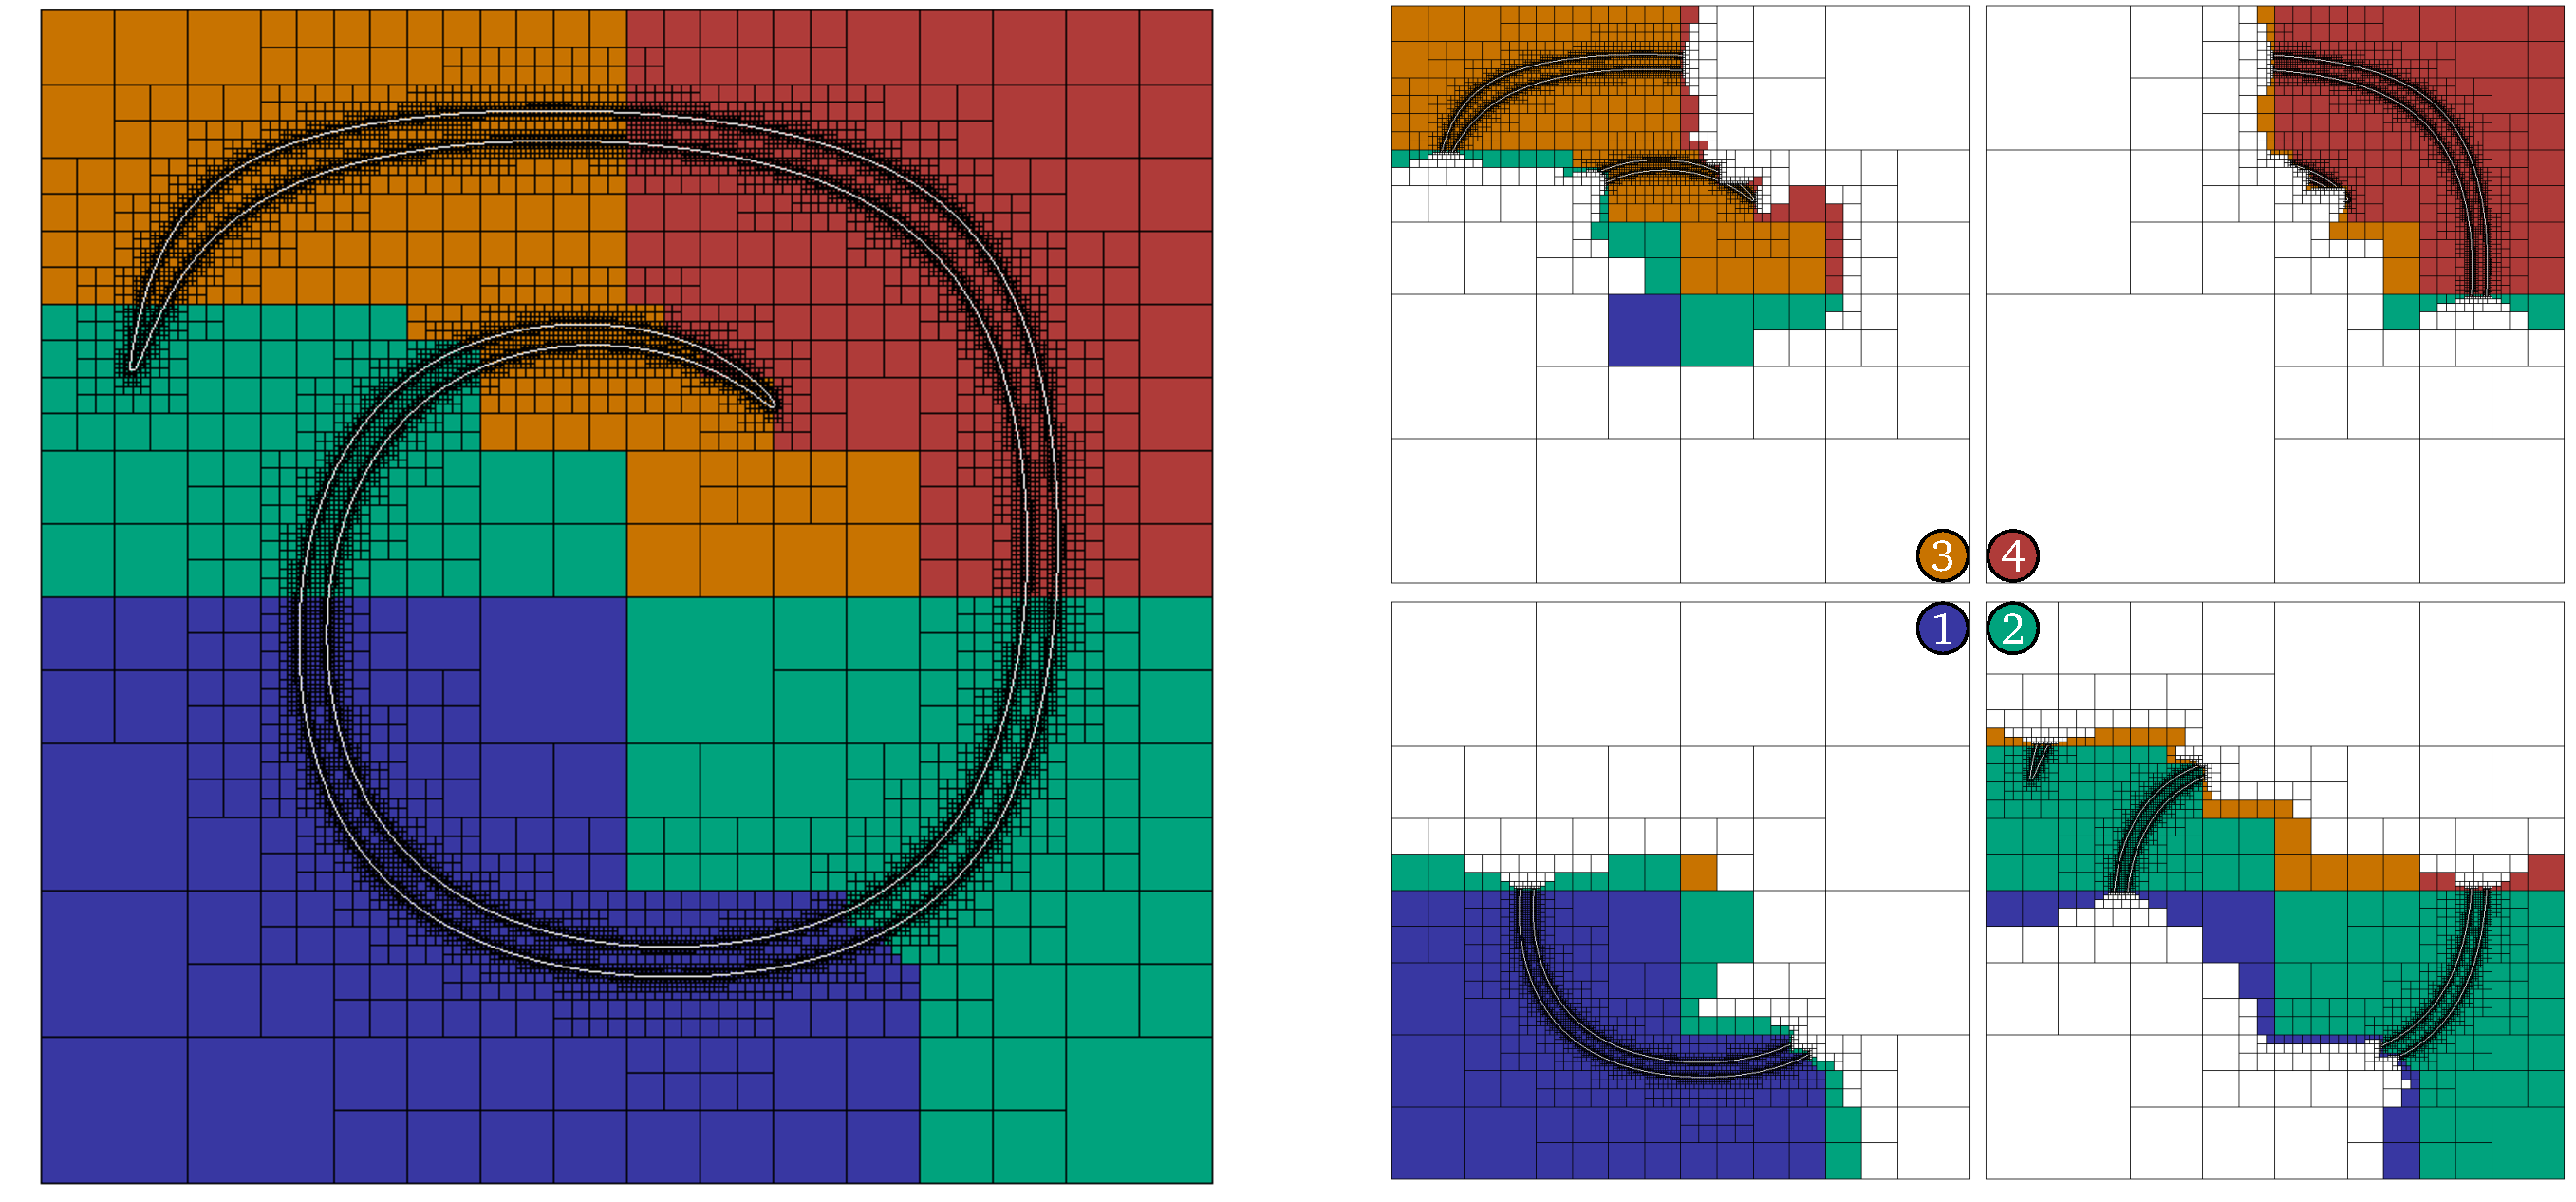
\includegraphics[width = \textwidth]{figures/reconstruct.pdf}
\end{center}
\caption{Left: A forest refined close to an interface and partitioned among four processors as indicated by colors. Right: Each processor independently recreates a local forest which is refined to match the global grid and is as coarse as possible elsewhere. Note that empty cells are fictitious, i.e. they are only required to generate the hierarchal structure and are not matched by any corresponding cell in the global forest.}
\label{fig:reconstruction}
\end{figure}

\subsection{Semi-Lagrangian method}
As indicated earlier, we use the Semi-Lagrangian method to solve equation \eqref{eq:ls} when the velocity field is externally generated, i.e. does not depend on level-set function itself. Let us rewrite equation \eqref{eq:ls} along the characteristic curve $\mathbf{X}(t)$ as:
\be
\left\{
\begin{array}{rcl}
\dfrac{\text{d} \mathbf{X}}{\text{d} t} &=& \mathbf{V}, \\ [3ex]
\dfrac{\text{d} \phi(\mathbf{X}(t), t)}{\text{d} t} &=& 0.
\end{array}
\right.
\label{eq:sl}
\ee
The Semi-Lagrangian method integrates equations \eqref{eq:sl} backward in time, i.e. starting from the grid $G^{n+1}$ \footnote{$G^{n+1}$ itself is computed in an iterative fashion as explained later on.}, we simply write $\phi^{n+1}(\mathbf{X}^{n+1}) = \phi(\mathbf{X}(t^{n+1}), t^{n+1}) = \phi(\mathbf{X}(t^n), t^n) = \phi^n(\mathbf{X}_d)$. Here the characteristic curves are chosen such that $\mathbf{X}(t^{n+1})$ are simply the coordinates of grids points of $G^{n+1}$. Moreover $\mathbf{X}_d$ are the departure points which are computed using the second-order midpoint method \cite{Min;Gibou:07:A-second-order-accur}:
\bea
\mathbf{X}^\star &=& \mathbf{X}^{n+1} - \frac{\Delta t}{2} \mathbf{V}^{n}(\mathbf{X}^n),	   \label{eq:xstar}      \\
\mathbf{X}_d     &=& \mathbf{X}^{n+1} - \Delta t \mathbf{V}^{n+\frac{1}{2}}(\mathbf{X}^\star), \label{eq:xdeparture}
\eea
where $\mathbf{V}^{n+\frac{1}{2}}$ is obtained via extrapolation from previous times, i.e.:
\be
\mathbf{V}^{n+\frac{1}{2}} = \frac{3}{2} \mathbf{V}^n - \frac{1}{2}\mathbf{V}^{n-1}. \label{eq:vn_p_half}
\ee

Note that all values at the intermediate point, $\mathbf{X}^\star$, and departure point, $\mathbf{X}_d$, must be calculated via interpolation from previous grids, $G^{n}$ and $G^{n-1}$. Here we use the stabilized second-order interpolation for $\phi(\mathbf{X}_d)$ and the multi-linear interpolation for $\mathbf{V}^{n+\frac{1}{2}}(\mathbf{X}^\star)$ \cite{Min;Gibou:07:A-second-order-accur}. Although parallelization of the interpolation process on a shared-memory machine is trivial, the same cannot be said for distributed-memory machines. In fact, the parallel interpolation algorithm \ref{alg:interpolation} is probably the most important contribution of this article. Complication arises because not all calculated departure points will reside in the domain of current processor. Moreover, due to the irregular shape of partitions, we cannot be certain that they are entirely owned by neighboring processors. At best we can only expect that their location are bounded by a halo of width $w \le \text{CFL} \: \Delta x_{\min}$ around the local partition. Of course if one enforces $\text{CFL} \le 1$, one can ensure that the halo is bounded by the ghost layer which significantly simplifies the communication problem. This assumption, however, defeats the purpose of using Semi-Lagrangian in the first place since we are interested in large values of $\text{CFL}$ number.

One remedy to this problem, proposed in \cite{Thomas;Cote:95:Massively-parallel-s} for uniform grids, is to increase the size of ghost layer to $\lceil \text{CFL} \rceil$. For large values of $\text{CFL}$ number, however, this approach can substantially increase the communication volume. Moreover, this simple approach does not work in the process of generating $G^{n+1}$ due to repartitioning. An alternative approach would be to handle local and remote interpolations separately. Our remote interpolation algorithm is composed of three separate phases. In the first phase, which we call buffering, every processor searches for all departure points inside the local tree. If the point is owned by a local cell, it is added to a local buffer, otherwise we find the processor which owns the point and add the point to a separate buffer belonging to the found rank. Note that searching the point in the local tree is performed recursively, similar to the \texttt{UpdateLocalTree} function in algorithm \ref{alg:reconstruction}. The owner's rank is found by computing the Z-index of the point and then using binary search on the Z-curve. This is already implemented in \texttt{p4est} and explained in details in section 2.5 of \cite{Burstedde;Wilcox;Ghattas:11:p4est:-Scalable-Algo}.

Once buffering is done, every processor knows exactly how many messages it needs to send and to which processors. This also implicitly defines processors that will later on send a reply message to this processor. However, at this point no one knows which processors they should expect a message from. We solve this problem using a simple \textit{communication matrix} (see figure \ref{fig:communication}). Other approaches for solving this problem could include using non-blocking collective or one-sided communication operations introduced in the MPI-3 standard \cite{MPI_ref, sparse dynamic exchange protocol paper}. Although these algorithms have better theoretical communication complexities, we did not see any difference in the runtime or scalability of algorithm \ref{alg:interpolation} when using them. 

\begin{figure}[htbp]
\begin{center}
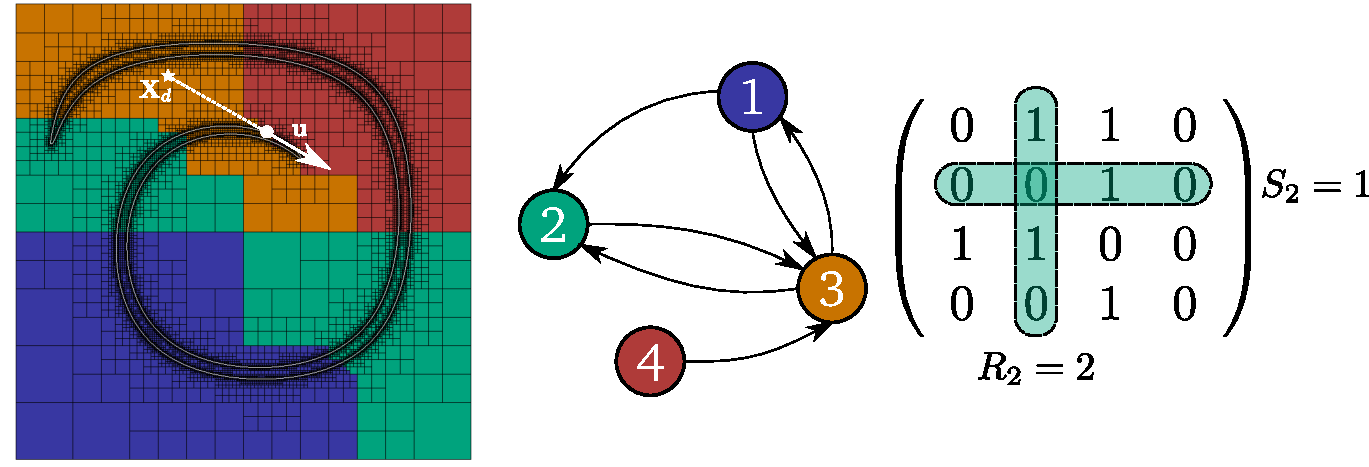
\includegraphics[width = \textwidth] {figures/communication.pdf}
\end{center}
\caption{Left: Location of back-traced points depends on the magnitude of local velocity and time-step. Although departure distance is bounded by $\text{CFL} \: \Delta x_{\min}$, one cannot make any special assumption about receiving rank without explicit searching of the entire Z-curve. Moreover, the receiving processor has no prior knowledge about which processors to check for incoming messages nor does it know anything about the possible message length (i.e. number of points). Middle: A directed graph illustrating the communication pattern among processors with arrows representing the direction that messages are sent. Right: The adjacency matrix of communication graph. For each row, sum of all columns represents the number of sent messages. Conversely, for each column, sum of all rows represents number of messages that need to be received. As detailed in algorithm \ref{alg:interpolation} this information is enough to build a parallel interpolation scheme.}
\label{fig:communication}
\end{figure}

To solve the communication problem, we first compute the adjacency matrix of the communication pattern, i.e. we construct the matrix $A_{P \times P}$ such that:
\ben
a_{ij} = 
\left\{
\begin{array}{lr}
1 \hspace{5 mm} \text{if processor `\textit{i}' sends a message to processor `\textit{j}',} \\
0 \hspace{5 mm} \text{otherwise.}
\end{array}
\right.
\een
Note that this matrix is also distributed among processors, i.e. each row is owned by a separate rank. Next, we compute:
\ben
S_i = \sum_j a_{ij} \hspace{5 mm} \text {and} \hspace{5 mm} R_i = \sum_j a_{ji}
\een
where $S_i$ and $R_i$ denote the number of sent and received messages respectively. While $S_i$ can be computed trivially, a reduction operation is required for computing $R_i$. For instance, this can be achieved using a single \texttt{MPI\_Reduce\_scatter} function call. The last phase of interpolation involves overlapping the computation of interpolated values for local points with the communication of data between processors. This is done by alternating between local calculations and probing for incoming messages from other processors. Interpolation is finished once values for all local points have been calculated and all remote requests have been processed (see algorithm \ref{alg:interpolation}).
\begin{algorithm}[htbp]
\caption{$values \gets \texttt{Interpolate (}H, \mathbf{X}\texttt{)}$}\label{euclid}
\begin{algorithmic}[1]
\State $col \gets 0, buff \gets null$ \Comment{Phase I -- buffering}
\For {$\mathbf{p} : \mathbf{X}$} 
	\State $[r, cell] \gets H.\texttt{search(}\mathbf{p}\texttt{)}$ \Comment{search for the owner's rank and cell}
	\If {$r = mpirank$}
		\State $buff[r].\texttt{push\_back(}\mathbf{p}, cell\texttt{)}$
	\Else
		\State $buff[r].\texttt{push\_back(}\mathbf{p}\texttt{)}$
		\State $col[r] \gets 1$
	\EndIf
\EndFor
\For {$r: mpisize$} \Comment{Phase II -- initiate communication and compute number of messages}
	\If {$col[r]$}
		\State $\texttt{MP\_Isend(}r, buff[r]\texttt{)}$
	\EndIf
\EndFor
\State  $S \gets \texttt{sum(}col\texttt{)}$ 
\State  $R \gets \texttt{MPI\_Reduce\_scatter(}col,\texttt{MPI\_SUM)}$
\State $done \gets false, it \gets buff[mpirank].\texttt{begin()}$
\While {$!done$} \Comment{Phase III -- main loop}
	\If {$it \not= buff[mpirank].\texttt{end()}$}
		\State $values \gets \texttt{process\_local(}it\texttt{)}$ \Comment{process local interpolations}
		\State $\texttt{++}it$
	\EndIf
	\If {$R > 0$} \Comment{process queries sent from remote processors}
		\State $[msg, st] \gets \texttt{MPI\_Iprobe()}$
		\If {$msg$}
			% \State $values \gets \texttt{MPI\_Recv(}st.\texttt{MPI\_SOURCE)}$ \Comment{}
			\State $val\_buff \gets \texttt{process\_queries(}st\texttt{)}$ \Comment{receive, search, and interpolate values}
			\State $\texttt{MPI\_Isend(}st.\texttt{MPI\_SOURCE},val\_buff\texttt{)}$ \Comment{send back interpolated values}
			\State $R\texttt{--}$
		\EndIf
	\EndIf
	\If {$S > 0$} \Comment{process replies sent to our queries}
		\State $[msg, st] \gets \texttt{MPI\_Iprobe()}$
		\If {$msg$}
			\State $values \gets \texttt{process\_replies(}st.\texttt{MPI\_SOURCE)}$ \Comment{receive remotely interpolated values}
			\State $S\texttt{--}$
		\EndIf
	\EndIf
	\State $done \gets S = 0 \: \And \: R = 0 \: \And \: it = buff[mpirank].\texttt{end()}$
\EndWhile
\State \Return $values$
\end{algorithmic}
\label{alg:interpolation}
\end{algorithm}

Using the interpolation algorithm \ref{alg:interpolation}, we close this section by presenting the final Semi-Lagrangian algorithm \ref{alg:semi-lagrangian}. The basic idea here is to start from an initial guess $G^{n+1}_0$ and modify the grid using refinement and coarsening criteria in \eqref{eq:refine} and \eqref{eq:coarsen} until convergence is obtained. Various options are available for $G^{n+1}_0$. For instance it is possible to start from the macromesh and only perform refinement steps until convergence. This choice, however, is not suitable since first few iterations do not contain many cells and there is little work for parallelism. Here we simply take the previous grid as the starting point, i.e. $G^{n+1}_0 = G^n$. Note that this iterative process is essentially unavoidable since the grid is based on the value of the level-set function at $t^{n+1}$, which itself is unknown and is to be defined on $G^{n+1}$. Nonetheless the process converges to the final grid in at most $l_{\max}$ steps where $l_{\max}$ denotes the maximum final depth of trees across all processors.
\begin{algorithm}[htbp]
\caption{$[G^{n+1}, \phi^{n+1}] \gets \texttt{SemiLagrangian (}G^n, \phi^n, \mathbf{V}^n, \mathbf{V}^{n-1}, \text{CFL}\texttt{)}$}\label{euclid}
\begin{algorithmic}[1]
\State $\Delta t_l \gets \text{CFL} \times \max \{\mathbf{V}^n\} / G^n.\texttt{hmin()}$
\State $\Delta t   \gets \texttt{MPI\_Allreduce(}\Delta t_l,\texttt{MPI\_MIN)}$
\State $H^n \gets \texttt{Reconstruct(} G^n\texttt{)}$ 
\State $G^{n+1}_0 \gets G^n$
\While {$true$}
	\State $\mathbf{X}_d  \gets \texttt{ComputeDeparturePoints(}G^{n+1}_0, \mathbf{V}^n, \mathbf{V}^{n-1}, \Delta t\texttt{)}$ \Comment{using equations \ref{eq:xstar} -- \ref{eq:vn_p_half}}
	\State $\phi^{n+1} \gets \texttt{Interpolate(}H^n, \textbf{X}_d\texttt{)}$
	\State $G^{n+1} \gets G^{n+1}_0.\texttt{refine\_and\_coarsen(}\phi^{n+1}\texttt{)}$ \Comment{using equations \ref{eq:refine} and \ref{eq:coarsen} as criteria}
	\If {$G^{n+1} \not= G^{n+1}_0$}
		\State $G^{n+1}.\texttt{partition()}$
		\State $G^{n+1}_0 \gets G^{n+1}$
	\Else
		\State \textbf{break}
	\EndIf
\EndWhile

\State \Return $[G^{n+1}, \phi^{n+1}]$
\end{algorithmic}
\label{alg:semi-lagrangian}
\end{algorithm}

\subsection{Reinitialization}
Successive application of algorithm \ref{alg:semi-lagrangian}, especially for large values of CFL number, potentially lead degrades the signed distance property of level-set function. It is thus important to reinitialize the level-set every few iterations, especially because the quality of generated grid heavily depends on the signed distance property. To achieve this property we solve the pseudo-time transient equation \eqref{eq:reinitialization} using the discretization scheme detailed in \cite{Min;Gibou:07:A-second-order-accur}. For completeness, we briefly review the scheme here. First equation \eqref{eq:reinitialization} is written in the following semi-discrete form:
\be
\frac{\text{d} \phi}{\text{d} \tau} + S(\phi_0) \left(\mathcal{H}_G(D^+_i \phi, D^-_i \phi) - 1 \right) = 0,
\label{eq:semidiscrete_reinit}
\ee
where $D^+_i \phi$ and $D^-_i \phi$ are the forward and backward derivatives in the $x_i$ direction and $\mathcal{H}_G$ is the Godunov Hamiltonian defined as:\
\ben
\mathcal{H}_G(a_i, b_i) = 
\left\{
\begin{array}{lcr}
	\sqrt{\sum_i \max\left(|a^+_i|^2, |b^-_i|^2\right)} & \hspace {5 mm} \text{if} & S(\phi_0) \le 0 \\
	\\
	\sqrt{\sum_i \max\left(|a^-_i|^2, |b^+_i|^2\right)} & \hspace {5 mm} \text{if} & S(\phi_0)  >  0 
\end{array}
\right.
,
\een
where $a^+ = \max(a, 0)$ and $a^- = \min(a, 0)$. Similar to \cite{Min;Gibou:07:A-second-order-accur}, equation \eqref{eq:semidiscrete_reinit} is integrated in time using the TVD-RK2 scheme using adaptive time-stepping to accelerate convergence to steady state. Since all computation is grid based, parallel implementation of this scheme is mostly trivial. However, one minor point requires further explanation. As suggested in \cite{Min;Gibou:07:A-second-order-accur}, one-sided derivatives $D^+_i \phi$ and $D^-_i \phi$ are computed using second order discretizations which require computation of second derivatives. To enable overlap between computation and communications when computing second derivatives and also integrating \eqref{eq:semidiscrete_reinit}, we use the following common technique. First, we label all local points, $L_p$, as either private, $P_p$, or boundary, $B_p$. Here, boundary points are the collection of all local points that are regarded as ghost point, $G_r$, on all other processors, i.e. $B_p = \underset{r,\;r\neq p}{\bigcup} G_r$. Private points are fined as the collection of all local points that are not a boundary point, i.e. $P_p = L_p \setminus B_p$. Algorithm \ref{alg:overlap} illustrates how this labeling can help with computation/computation overlap of an arbitrary local operation $\phi^{n+1} \gets \mathcal{F}(\phi^n)$. Note that \texttt{p4est} library already includes all the primitives required for labeling local points without any further communication.

\begin{algorithm}[htbp]
\caption{$\phi^{n+1} \gets \texttt{Overlap (}\phi^n, \mathcal{F}\texttt{)}$}\label{euclid}
\begin{algorithmic}[1]
\For {$i:B_p$} \Comment{I -- perform computation on boundary points}
	\State $\phi^{n+1}_i \gets \mathcal{F}(\phi_i^n)$
\EndFor
\State $send\_req \gets \texttt{MPI\_Isend(}\phi^{n+1}_B\texttt{)}$ \Comment{II -- begin updating ghost values}
\State $recv\_req \gets \texttt{MPI\_Irecv(}\phi^{n+1}_G\texttt{)}$
\For {$i:P_p$} \Comment{III -- perform computation on private points}
	\State $\phi^{n+1}_i \gets \mathcal{F}(\phi_i^n)$ 
\EndFor
\State $\texttt{MPI\_Waitall(}send\_req, recv\_req\texttt{)}$ \Comment{IV -- finish updating ghost values}
\State \Return $\phi^{n+1}$
\end{algorithmic}
\label{alg:overlap}
\end{algorithm}
% %!TEX root = draft.tex
\section{Scaling results} \label{sec:scaling}
In this section we present some results that demonstrate the scalability of our algorithms. All of our tests were ran on the Stampede cluster at the Texas Advanced Computing Center (TACC) where we are limited to $4096$ cores at most. Each node of Stampede has 2 eight-core Xenon E5-2680 processes clocked at 2.7 GHz with 32 GB of DDR3-1600 MHz memory and interconnected using an InfiniBand network card. Unless mentioned otherwise, in all the tests we have used all 16 cores of every node. Finally, in all cases we report the maximum wall time recorded using PETSc's logging interface which has a temporal resolution of roughly $0.1 \: \mu s$.

We define parallel efficiency as $e=s\cdot P_1 / P$ where $s=t_1/t_P$ is the speed-up, $P_1$ is the smallest number of processes for which the test was run, $t_1$ is the time to run the problem on $P_1$ processes, $P$ is the number of processes and $t_P$ is the time to run the problem on $P$ processes. We note that efficiencies larger than $100\%$ are reported for some cases. This is common and can be hardware related, for instance linked to the problem being locally smaller for larger number of processes and thus exploiting the cache better.

\subsection{Interpolation}
In this section we show the results for a simple test to measure the scalability of the interpolation Algorithm \ref{alg:interpolation}. The test consists of interpolating a function at a number of random points on a randomly refined Octree in three spatial dimensions. We consider two cases, a small test on a level\footnote{The level is the number of recursive splits allowed for each tree.} 9 tree with roughly 33M nodes and a larger test on a level 13 tree with roughly 280M nodes. In both cases the number of randomly generated points is chosen to be equal to the number of nodes and the stabilized second-order interpolation of \cite{Min;Gibou:07:A-second-order-accur} is performed 10 times to smooth out possible timing fluctuations.

To simulate the effect of different CFL numbers, we generate the random points such that on each process $\alpha$ percentage of them are located outside the process boundary and thus will initiate communication. Scaling results are presented for $\alpha = 5 \%$ and $\alpha = 95\%$ for both the small and large problems in Figure \ref{fig:interpolation}. We also present a third row of results for a much larger problem with roughly 1.66B nodes on a level 14 tree. Excellent scaling is obtained for the small problem for $P = 16-512$ even when $95\%$ of the interpolation points belong to a remote process. For the larger problem, however, the communication overhead prevents the algorithm from scaling beyond $2048$ processes when $\alpha = 95\%$ (cf.\ Table \ref{tab:scaling_interpolation}). Note, however, that this is expected since the total time is dominated by communication for $\alpha = 95\%$ and there is very little local work in this case. Indeed, the last row of Figure \ref{fig:interpolation} show much better scaling behavior on a larger problem size, e.g. efficiencies are increased from $e=34\%$ to $e=68\%$ for $\alpha = 95\%$ on 4096 processes. This is a typical result with strong scaling and simply implies that our algorithms are scalable for sufficiently large problems.
\begin{figure}[htbp]
	\begin{center}
		\subfigure[$N_G = 33$M, $\alpha = 5\%$]{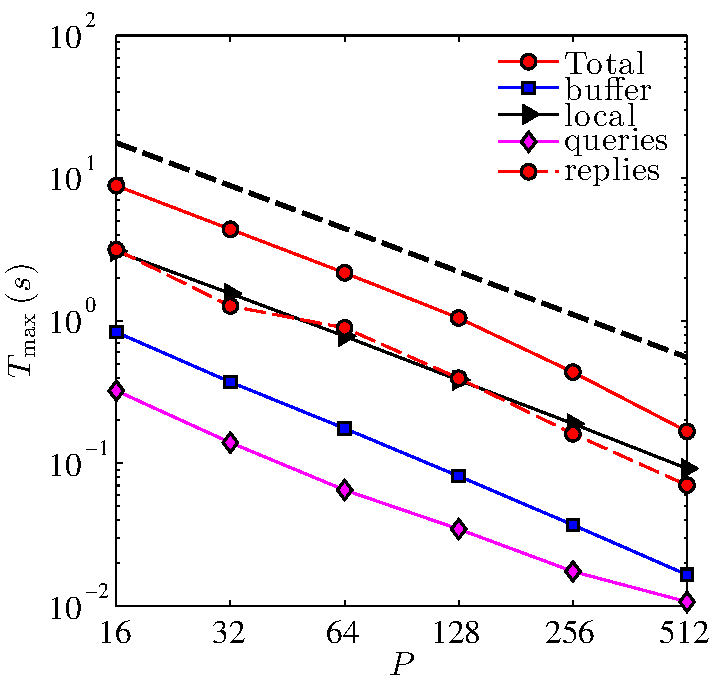
\includegraphics[width = 0.38 \textwidth] {figures/host_Interpolation_small_alpha_5.pdf}} \hspace{0.5 in}
		\subfigure[$N_G = 33$M, $\alpha = 95\%$]{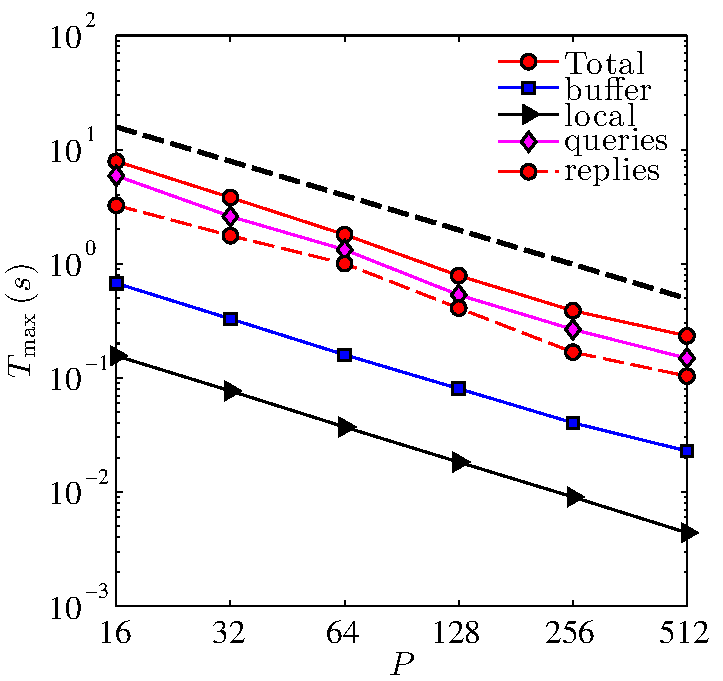
\includegraphics[width = 0.38 \textwidth] {figures/host_Interpolation_small_alpha_95.pdf}}
		\\
		\subfigure[$N_G = 280$M, $\alpha = 5\%$]{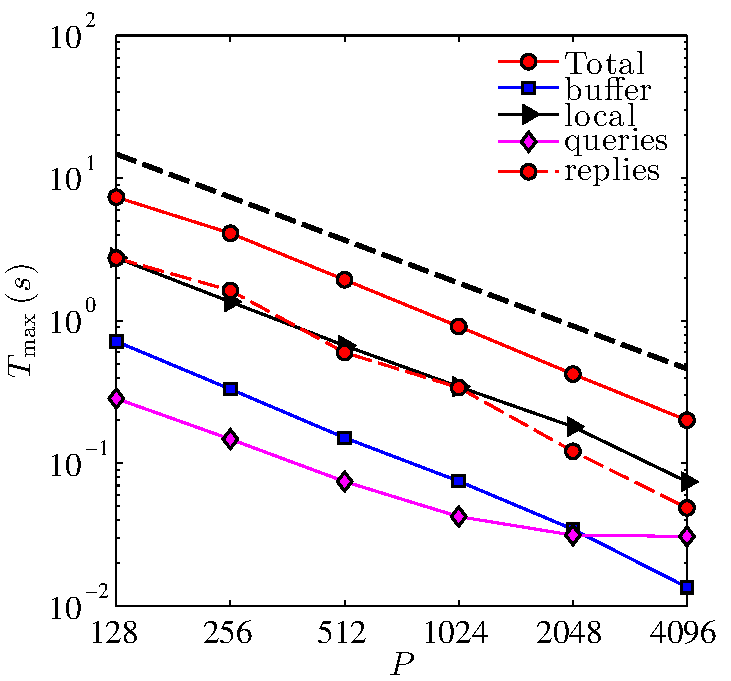
\includegraphics[width = 0.38 \textwidth] {figures/host_Interpolation_large_alpha_5.pdf}} \hspace{0.5 in}
		\subfigure[$N_G = 280$M, $\alpha = 95\%$]{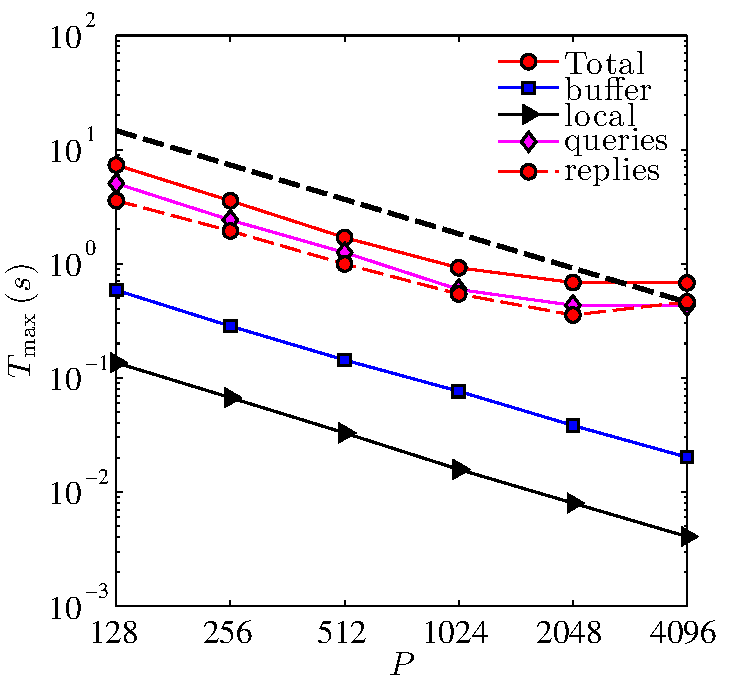
\includegraphics[width = 0.38 \textwidth] {figures/host_Interpolation_large_alpha_95.pdf}}
		\\
		\subfigure[$N_G = 1.66$B, $\alpha = 50\%$]{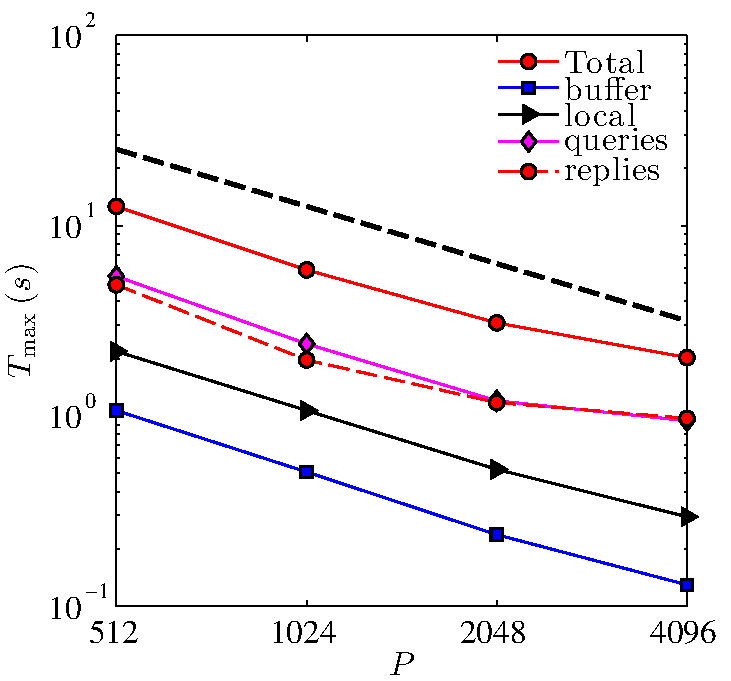
\includegraphics[width = 0.38 \textwidth] {figures/host_Interpolation_super_large_alpha_50.pdf}} \hspace{0.5 in}
		\subfigure[$N_G = 1.66$B, $\alpha = 95\%$]{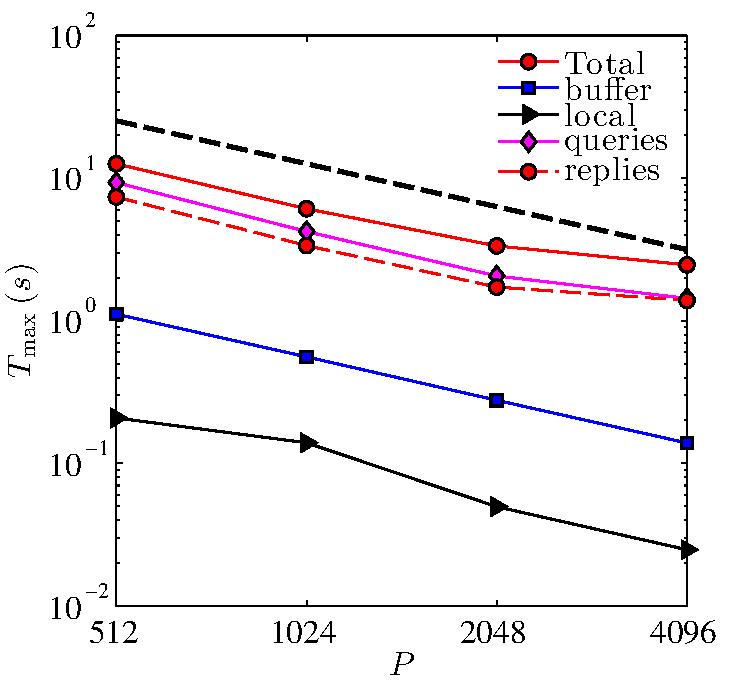
\includegraphics[width = 0.38 \textwidth] {figures/host_Interpolation_super_large_alpha_95.pdf}}
	\end{center}
	\caption{Strong scaling of Algorithm \ref{alg:interpolation} for several tests where $N_G$ denotes the number of random interpolation points (which is the same as the number of nodes in the Octree) and $\alpha$ denotes the percentage of these points that are remote for each process. Here ``Total'' represents the total time spent in the interpolation while ``buffer'', ``local'', ``queries'', and ``replies'' represent the the timing for different sections (cf.\ Algorithm \ref{alg:interpolation}). The black dashed line represents the ideal scaling. The results indicate excellent scaling for the small test (a-b) and for the large test when $\alpha = 5\%$ (c). For the extreme case (d) the algorithm stops scaling at $2048$ processes due to communication overhead. Note, however, that this merely indicates that the problem size is not large enough for this test case. Indeed much better scaling is obtained when the problem size is increased to $N_G = 1.66$B points (e-f).}
	\label{fig:interpolation}
\end{figure}

\begin{table}[ht!]
\centering
	\begin{tabular}{|l|l|cccccc|}
	\hline
	\multirow{3}{*}{Small Test} & \multicolumn{1}{|c|}{$P$} & 16      & 32      & 64      & 128     & 256    & 512 \\
	\cline{2-8} 	                            
	                            & $\alpha = 5\%$   & $100\%$ & $101\%$ & $102\%$ & $106\%$ & $127\%$& $165\%$ \\
	                            & $\alpha = 95\%$  & $100\%$ & $104\%$ & $110\%$ & $125\%$ & $127\%$& $106\%$ \\ 	                            
	\hline
	\multirow{3}{*}{Large Test} & \multicolumn{1}{|c|}{$P$} & 128     & 256     & 512     & 1024    & 2048   & 4096 \\
	\cline{2-8} 	                            
	                            & $\alpha = 5\%$   & $100\%$ & $89\%$  & $95\%$  & $101\%$ & $109\%$& $114\%$ \\
	                            & $\alpha = 95\%$  & $100\%$ & $103\%$ & $108\%$ & $99\%$  & $67\%$ & $34\%$ \\
	\hline
	\multirow{3}{*}{Very Large Test} & \multicolumn{1}{|c|}{$P$} & 128     & 256     & 512     & 1024    & 2048   & 4096 \\
	\cline{2-8} 	                            
	                            & $\alpha = 50\%$  & -- & -- & $100\%$ & $108\%$ & $102\%$& $78\%$ \\
	                            & $\alpha = 95\%$  & -- & -- & $100\%$ & $103\%$ & $94\%$ & $64\%$ \\
	\hline
	\end{tabular}
	\caption{Parallel efficiency of the total runtime of the interpolation algorithm for the small (33M nodes), large (280M nodes), and very large (1.66B nodes) tests. Reported efficiencies are based on the lowest number of processes for each test.}
	\label{tab:scaling_interpolation}
\end{table}

\subsection{Semi-Lagrangian}
To test the scalability of the semi-Lagrangian scheme of Algorithm \ref{alg:semi-lagrangian}, we consider a slightly modified version of the Enright's rotation test \cite{Enright;Fedkiw;Ferziger;etal:02:A-Hybrid-Particle-Le} presented in section \ref{sec:accuracy}, i.e. we advect a sphere of radius 0.35 located at $(0.4, 0.4, 0.4)$ with a divergence free velocity field given by equation \eqref{eq:velo_enright}.

To understand the effect of the CFL number on the scalability of the algorithm we perform one step of the semi-Lagrangian algorithm for $\text{CFL} = 1$, $\text{CFL} = 10$, and $\text{CFL} = 100$. We also perform the test for two different initial girds, a small grid with maximum level $l_\text{max} = 10$ and a large grid with maximum level $l_\text{max} = 12$. In both cases, the minimum level is $l_\text{min}=0$. After one advection step, these grids have approximately 15M and 255M nodes, respectively. 
\begin{table}[htbp]
	\begin{minipage}{.48\linewidth}
		\begin{center}
		\begin{tabular}{|c|cccccc|}
			\hline
				\diagbox{CFL}{\#p} & 16 & 32 & 64 & 128 & 256 & 512 \\
				\hline
				1   & 2 & 2 & 3 & 3 & 3 & 3 \\
				10  & 3 & 3 & 3 & 3 & 3 & 3 \\
				100 & 6 & 6 & 6 & 6 & 6 & 6 \\
			\hline
		\end{tabular}
		\caption*{(a) $l_\text{max} = 10$}
		\end{center}
	\end{minipage}%
	\begin{minipage}{.48\linewidth}
		\begin{center}
		\begin{tabular}{|c|cccccc|}
			\hline
				\diagbox{CFL}{\#p} & 128 & 256 & 512 & 1024 & 2048 & 4096 \\
			\hline
				1   & 3 & 3 & 3 & 3 & 3 & 3 \\
				10  & 3 & 3 & 4 & 4 & 4 & 4 \\
				100 & 6 & 6 & 6 & 6 & 6 & 7 \\
			\hline
		\end{tabular}
		\caption*{(b) $l_\text{max} = 12$}
		\end{center}
	\end{minipage}	
	\caption{Number of sub-iterations required for the grid construction in Algorithm \ref{alg:semi-lagrangian} for the rotation test on a (a) level-10 and (b) level-12 Octree with approximately 15M and 255M nodes, respectively. Note how the sub-iteration count increases with the CFL number but is almost independent of the number of processes. The slight dependence between the number of sub-iterations and the number of processes is most likely due to the dependence of round-off errors on the number of processes. Nonetheless, close examination of the Octrees generated (data not shown) reveals that they are identical and independent of the number of processes used to perform the test.}
	\label{tab:semilagrangian}
\end{table}

Unlike many existing applications where the mesh is changed infrequently, our semi-Lagrangian algorithm requires several sub-iterations of the refinement and coarsening operations. As a result, it is expected that refinement and coarsening steps constitute a significant portion of the total runtime which puts stringent scalability requirements on these algorithms. We refer the interested reader to section 3.2 of \cite{Burstedde;Wilcox;Ghattas:11:p4est:-Scalable-Algo} for detailed description of scalable refinement and coarsening algorithms in \texttt{p4est}. 

Table \ref{tab:semilagrangian} illustrates the dependence of the number of sub-iterations required to build the grid on the CFL number; as the CFL is increased, the interface travels a farther distance, which necessitates more sub-iterations to generate the grid. Figures \ref{fig:semilagrangian_small} and \ref{fig:semilagrangian_large} illustrate the scalability of the algorithm for the small and large problems, respectively. To enable meaningful comparisons between different CFL numbers and number of processes, the maximum time has been scaled by the number of sub-iterations required for the grid construction as reported in Table \ref{tab:semilagrangian}. For both problems, excellent scalability is observed for $\text{CFL} = 1$ and $\text{CFL} = 10$. The algorithm even shows good scalability when taken to the extreme, i.e. for $\text{CFL} = 100$.

An increase in the CFL number has two effects on the algorithm. First, a larger fraction of the departure points lands in the domains of remote processes. Moreover, these points are potentially dispersed across a larger number of processes. This means that the communication volume should increase with the CFL number. Second, as more points are shipped to remote processes for interpolation, there is a greater chance that the interpolation load is imbalanced across processes. This is especially true for regions of space in which the streamlines cluster. Both factors can contribute to reducing the scalability of the algorithm at large CFL numbers. 
\begin{figure}[htbp]
	\begin{center}
		\subfigure[semi-Lagrangian, $\text{CFL} = 1$]{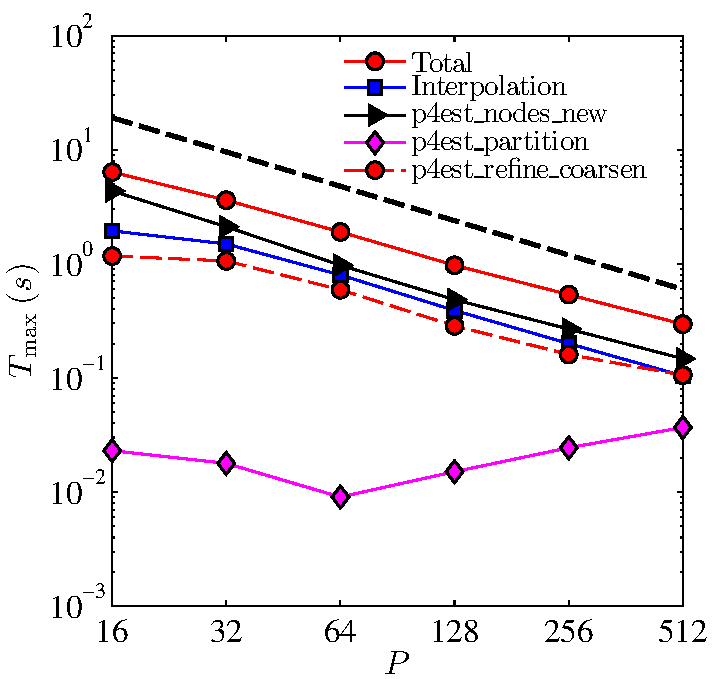
\includegraphics[width = 0.32 \textwidth] {figures/host_SemiLagrangian_small_CFL_1.pdf}}
		\subfigure[semi-Lagrangian, $\text{CFL} = 10$]{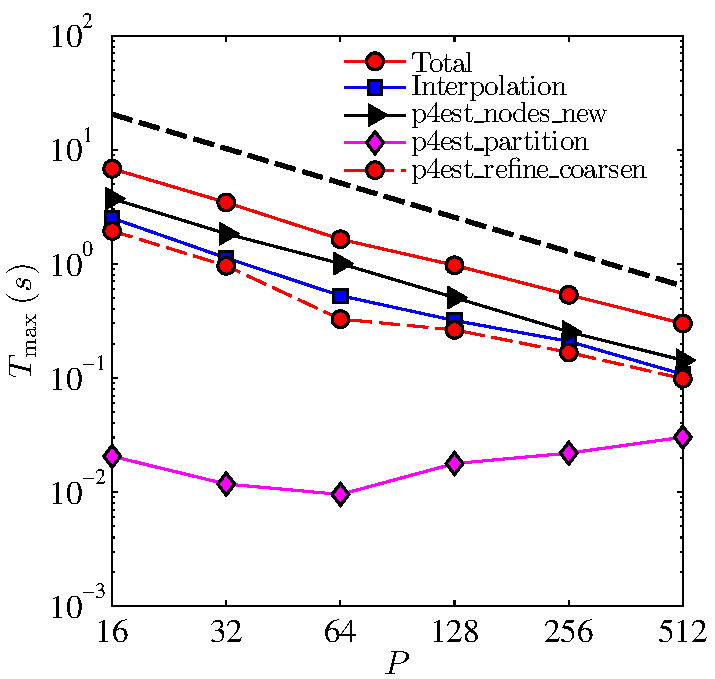
\includegraphics[width = 0.32 \textwidth] {figures/host_SemiLagrangian_small_CFL_10.pdf}}
		\subfigure[semi-Lagrangian, $\text{CFL} = 100$]{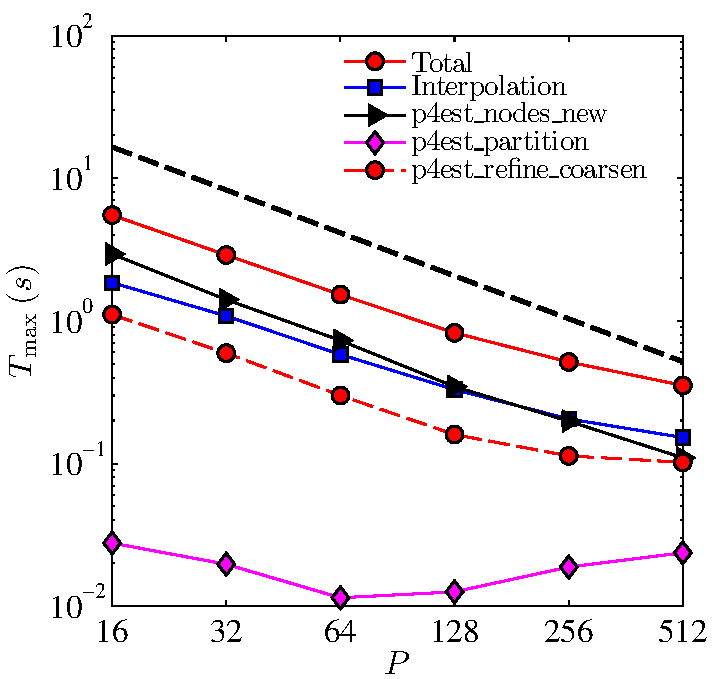
\includegraphics[width = 0.32 \textwidth] {figures/host_SemiLagrangian_small_CFL_100.pdf}}
		\\
		\subfigure[Interpolation, $\text{CFL} = 1$]{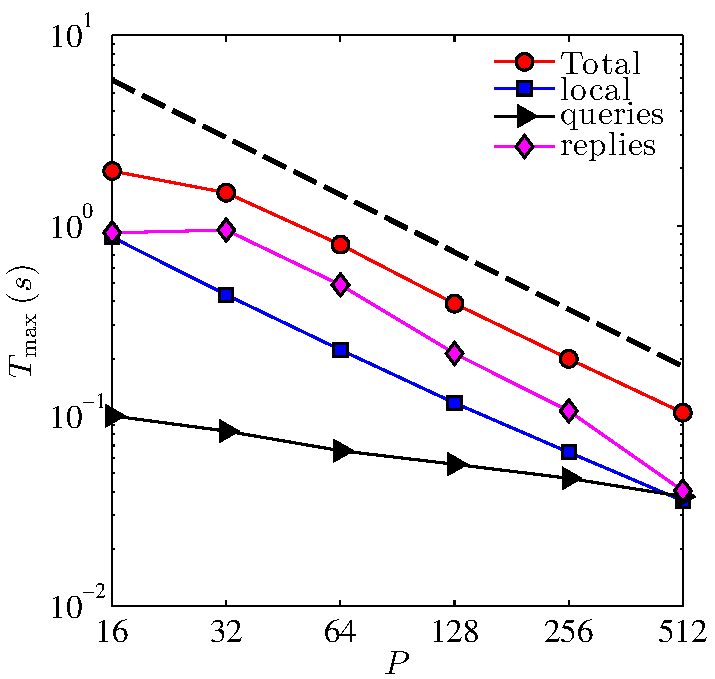
\includegraphics[width = 0.32 \textwidth] {figures/host_SemiLagrangian_Interpolation_small_CFL_1.pdf}}
		\subfigure[Interpolation, $\text{CFL} = 10$]{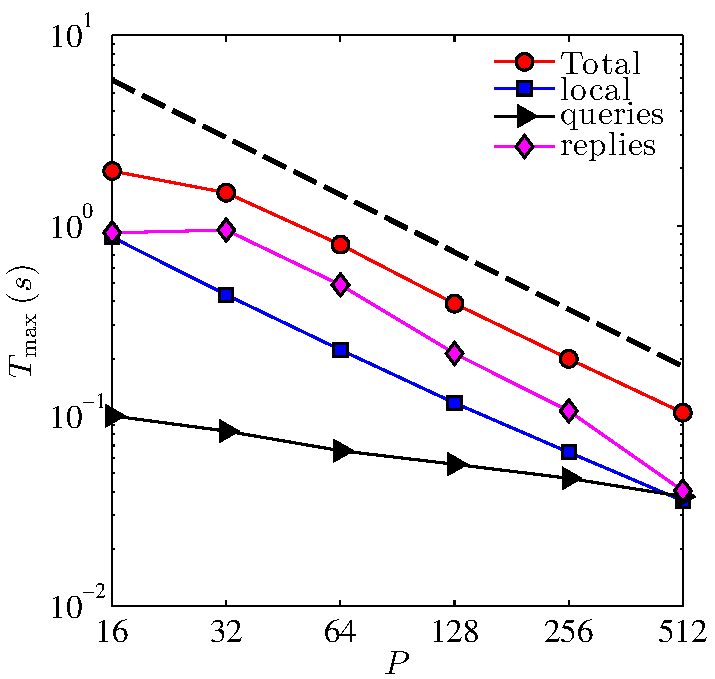
\includegraphics[width = 0.32 \textwidth] {figures/host_SemiLagrangian_Interpolation_small_CFL_1.pdf}}
		\subfigure[Interpolation, $\text{CFL} = 100$]{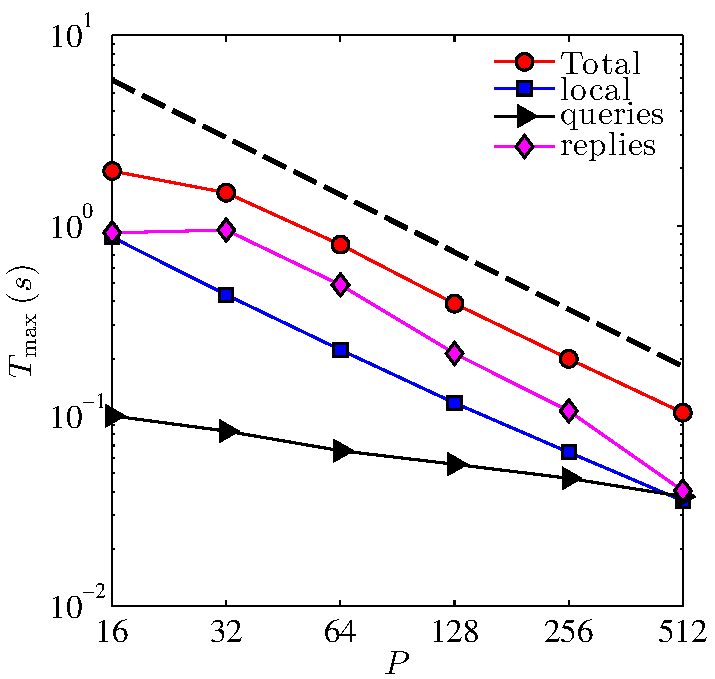
\includegraphics[width = 0.32 \textwidth] {figures/host_SemiLagrangian_Interpolation_small_CFL_1.pdf}}
	\end{center}
	\caption{Strong scaling of a single time step of Algorithm \ref{alg:semi-lagrangian} for the rotation test on a level-10 Octree with approximately 15M nodes. Top row: scaling of the various components of the algorithm for (a) $\text{CFL} = 1$, (b) $\text{CFL} = 10$, and (c) $\text{CFL} = 100$. Bottom row: breakdown of the various components of the interpolation phase for the same CFL numbers. The solid dashed line represents the ideal scaling. Note that the maximum time has been scaled by the number of sub-iterations required to build the tree (cf.\ Table \ref{tab:semilagrangian}). Here \texttt{p4est\_nodes\_new}, \texttt{p4est\_partition} and \texttt{p4est\_refine\_coarsen} refer to constructing the global indexing for nodes, partitioning the forest, and the refining/coarsening operation, respectively \cite{Burstedde;Wilcox;Ghattas:11:p4est:-Scalable-Algo}.}
	\label{fig:semilagrangian_small}
\end{figure}

\begin{figure}[htbp]
	\begin{center}
		\subfigure[semi-Lagrangian, $\text{CFL} = 1$]{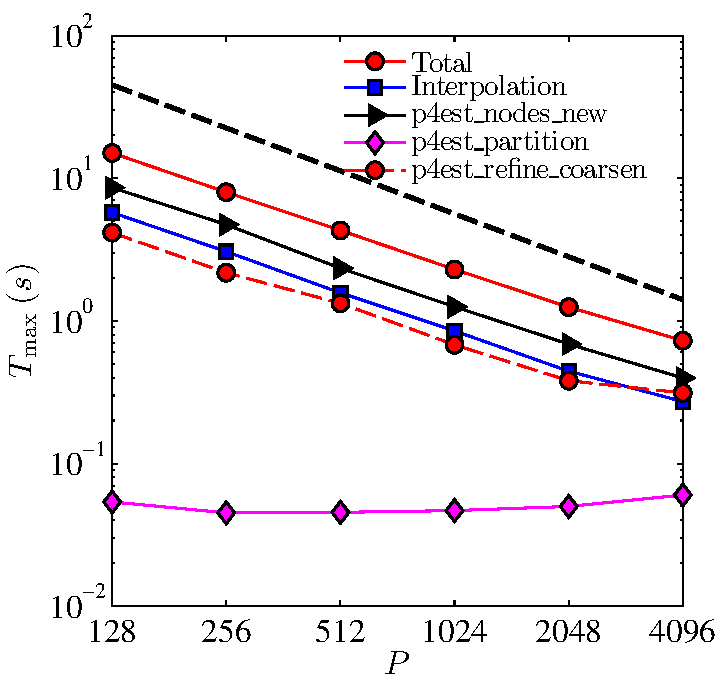
\includegraphics[width = 0.32 \textwidth] {figures/host_SemiLagrangian_large_CFL_1.pdf}}
		\subfigure[semi-Lagrangian, $\text{CFL} = 10$]{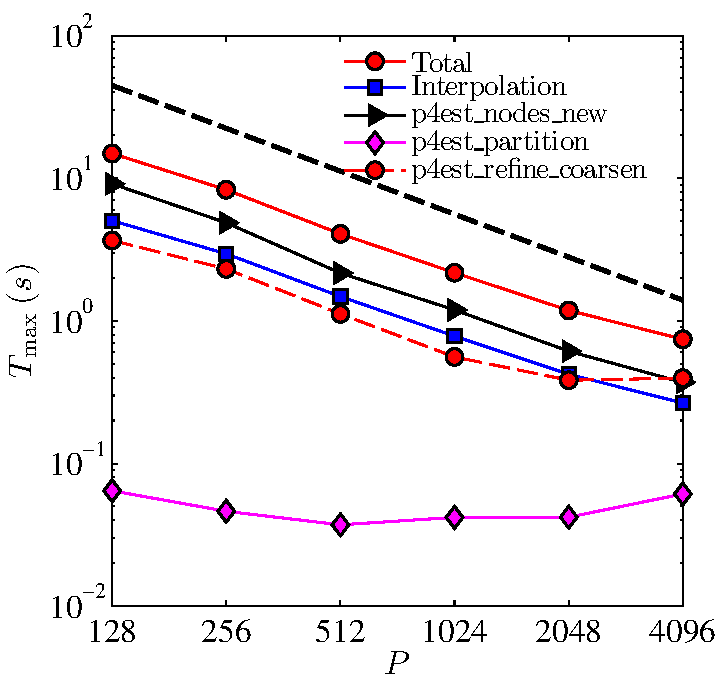
\includegraphics[width = 0.32 \textwidth] {figures/host_SemiLagrangian_large_CFL_10.pdf}}
		\subfigure[semi-Lagrangian, $\text{CFL} = 100$]{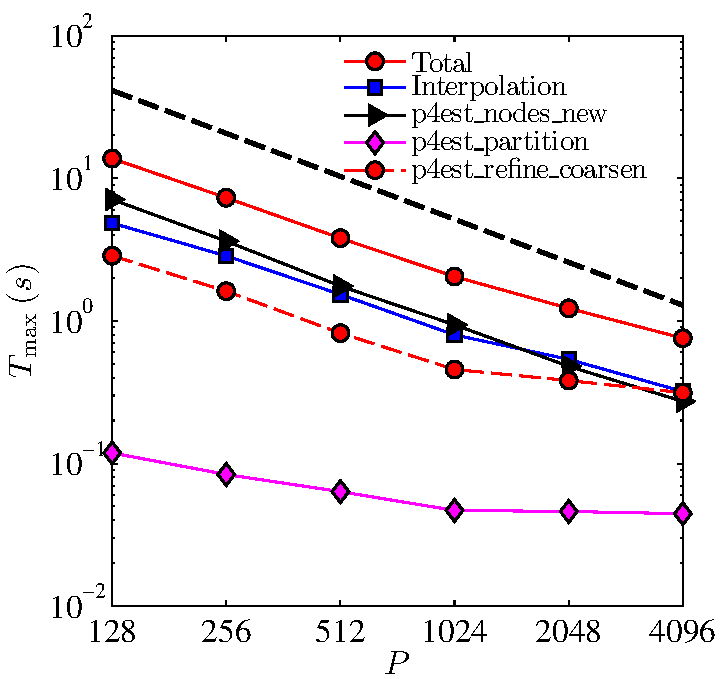
\includegraphics[width = 0.32 \textwidth] {figures/host_SemiLagrangian_large_CFL_100.pdf}}
		\\
		\subfigure[Interpolation, $\text{CFL} = 1$]{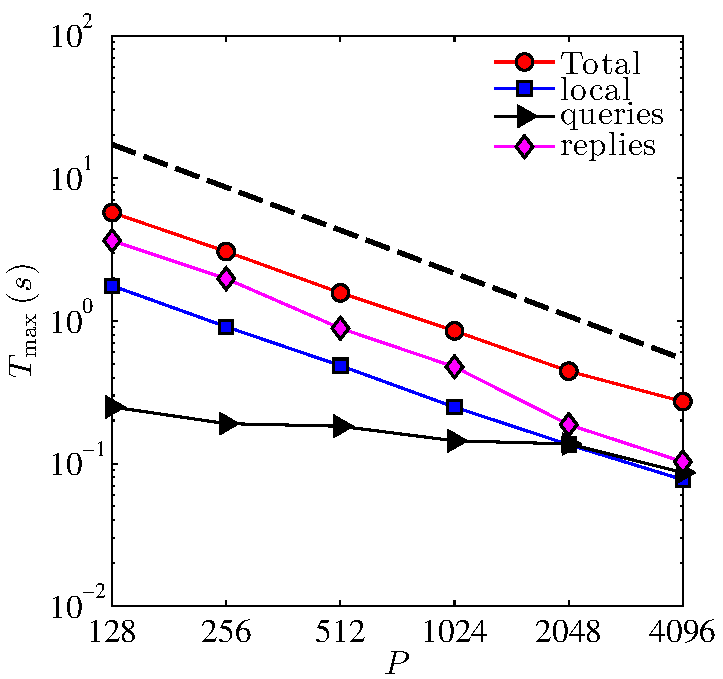
\includegraphics[width = 0.32 \textwidth] {figures/host_SemiLagrangian_Interpolation_large_CFL_1.pdf}}
		\subfigure[Interpolation, $\text{CFL} = 10$]{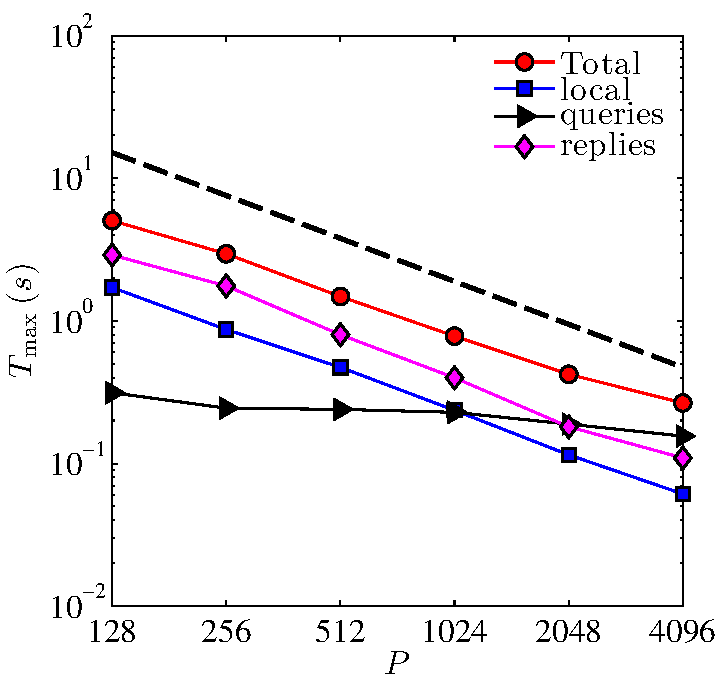
\includegraphics[width = 0.32 \textwidth] {figures/host_SemiLagrangian_Interpolation_large_CFL_10.pdf}}
		\subfigure[Interpolation, $\text{CFL} = 100$]{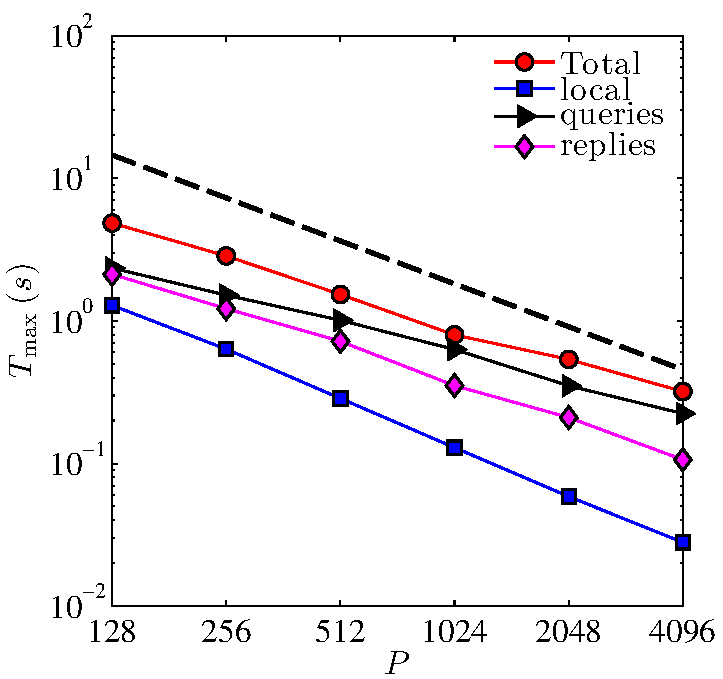
\includegraphics[width = 0.32 \textwidth] {figures/host_SemiLagrangian_Interpolation_large_CFL_100.pdf}}
	\end{center}
	\caption{Strong scaling of a single time step of Algorithm \ref{alg:semi-lagrangian} for the rotation test on a level-12 Octree with approximately 255M nodes. Top row: scaling of the various components of the algorithm for (a) $\text{CFL} = 1$, (b) $\text{CFL} = 10$, and (c) $\text{CFL} = 100$. Bottom row: breakdown of the various components of the interpolation phase for the same CFL numbers. The solid dashed line represents the ideal scaling. Note that the maximum time has been scaled by the number of sub-iterations required to build the tree (cf.\ Table \ref{tab:semilagrangian}).}
	\label{fig:semilagrangian_large}
\end{figure}

\begin{table}
\centering
	\begin{tabular}{|l|l|cccccc|}
	\hline
	\multirow{4}{*}{Small Test} & \multicolumn{1}{|c|}{$P$} & 16      & 32      & 64      & 128     & 256    & 512 \\
	\cline{2-8} 	                            
	                            & $\text{CFL} = 1$   & $100\%$ & $88\%$  & $84\%$  & $82\%$  & $74\%$ & $67\%$ \\
	                            & $\text{CFL} = 10$  & $100\%$ & $99\%$  & $104\%$ & $88\%$  & $80\%$ & $71\%$ \\ 	                            
	                            & $\text{CFL} = 100$ & $100\%$ & $95\%$  & $90\%$  & $84\%$  & $67\%$ & $49\%$ \\
	\hline
	\multirow{4}{*}{Large Test} & \multicolumn{1}{|c|}{$P$} & 128     & 256     & 512     & 1024    & 2048   & 4096 \\
	\cline{2-8} 	                            
	                            & $\text{CFL} = 1$   & $100\%$ & $94\%$  & $87\%$  & $82\%$  & $75\%$ & $65\%$ \\
	                            & $\text{CFL} = 10$  & $100\%$ & $90\%$  & $92\%$  & $86\%$  & $79\%$ & $63\%$ \\
	                            & $\text{CFL} = 100$ & $100\%$ & $94\%$  & $90\%$  & $84\%$  & $70\%$ & $57\%$ \\
	\hline
	\end{tabular}
	\caption{Parallel efficiency of the runtime of a single semi-Lagrangian step. Reported efficiencies are based on the lowest number of processes for each test.}
	\label{tab:scaling_semilagrangian}
\end{table}

To better understand the importance of the CFL number on the scalability, we have recorded a complete history of the communication pattern in the interpolation step. Figure \ref{fig:communication_4096} illustrates the effects of the CFL number on different metrics, namely the number of interpolation points\footnote{Note that this includes both the local points and the points queried by other processes.}, $N_p$, the number of sent and received messages, $N_m = S + R$, and the total communication volume, $V_m$ in megabytes (MB), for $p=4096$ processes. Furthermore, these values are reported for the first (top row) and last (bottom row) sub-iterations of the semi-Lagrangian algorithm. There are several points to make. First, increasing the CFL number greatly increases the load imbalance, as shown by the spread of the data in Figure \ref{fig:communication_4096_pf}. This is because at higher CFL numbers, it is more likely that some processes will receive a larger portion of the backtracked points. Second, increasing the CFL number increases both the communication volume and its spread across processes (cf.\ Figure \ref{fig:communication_4096_vf}). Interestingly, however, the number of sent and received messages do not seem to be affected by the CFL number. The bottom row of Figure \ref{fig:communication_4096} exhibits a better balance both in the computation and communication volume in the last sub-iteration of the semi-Lagrangian algorithm. This can be justified by noting that for the final sub-iteration, the partitioning of $G^{n+1}$ is more consistent with the partitioning of the departure points on $G^n$. Detailed information about the load balancing and the communication patterns is listed in Table \ref{tab:communication}.
\begin{figure}[htbp]
	\begin{center}
		\subfigure[]{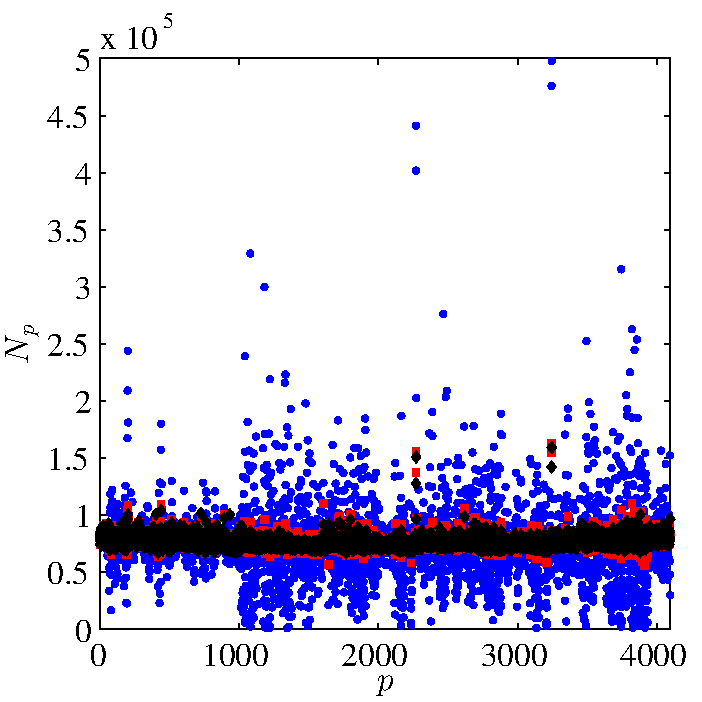
\includegraphics[width = 0.3 \textwidth] {figures/host_large_point_first_4096.pdf}  \label{fig:communication_4096_pf}}
		\subfigure[]{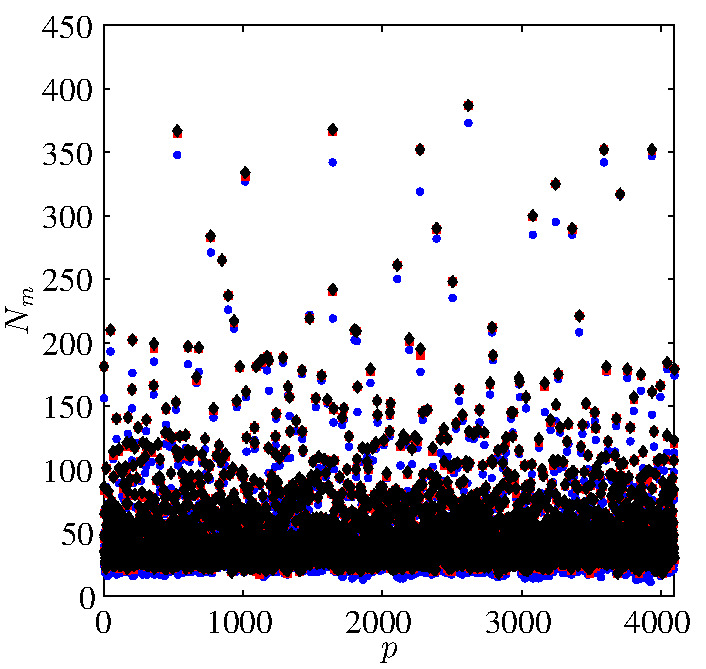
\includegraphics[width = 0.3 \textwidth] {figures/host_large_message_first_4096.pdf}\label{fig:communication_4096_mf}}
		\subfigure[]{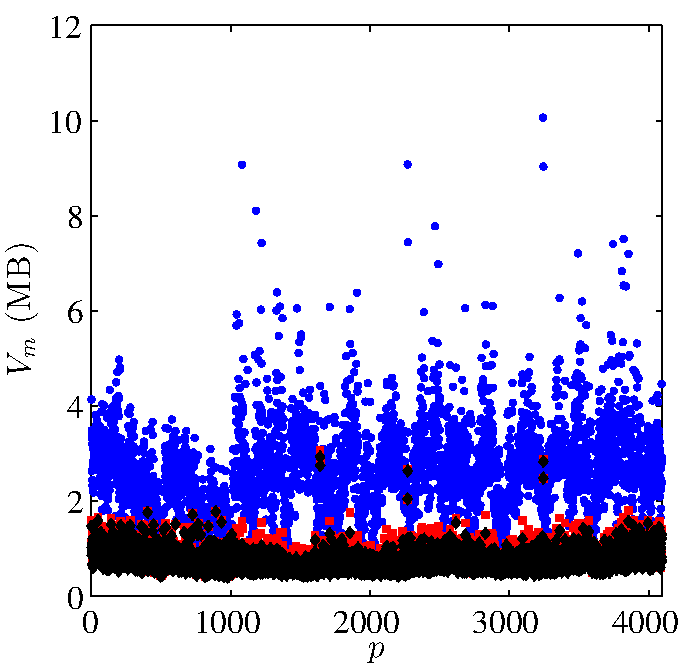
\includegraphics[width = 0.3 \textwidth] {figures/host_large_volume_first_4096.pdf} \label{fig:communication_4096_vf}}
		\\
		\subfigure[]{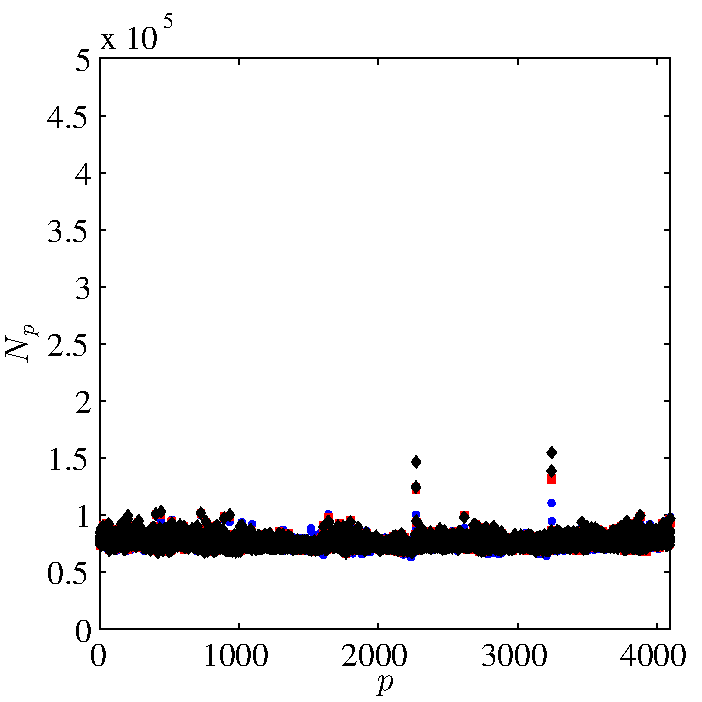
\includegraphics[width = 0.3 \textwidth] {figures/host_large_point_last_4096.pdf}   \label{fig:communication_4096_pl}}
		\subfigure[]{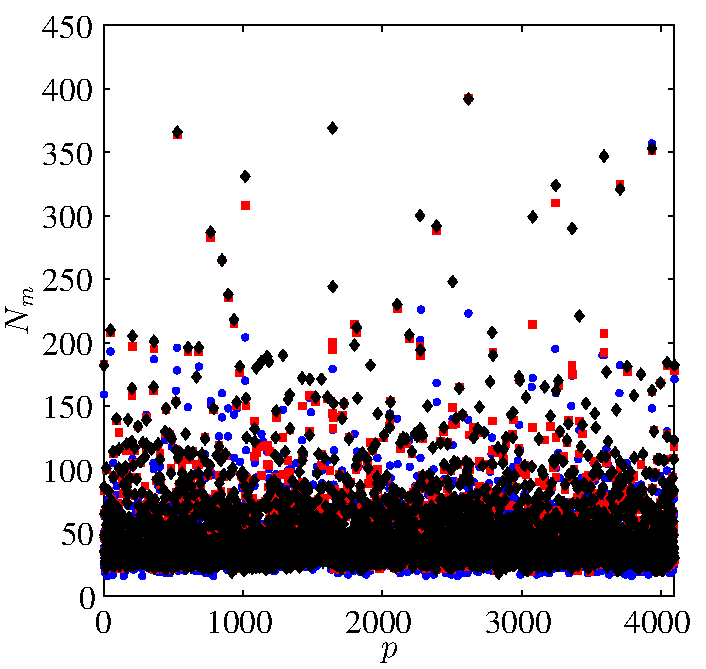
\includegraphics[width = 0.3 \textwidth] {figures/host_large_message_last_4096.pdf} \label{fig:communication_4096_ml}}
		\subfigure[]{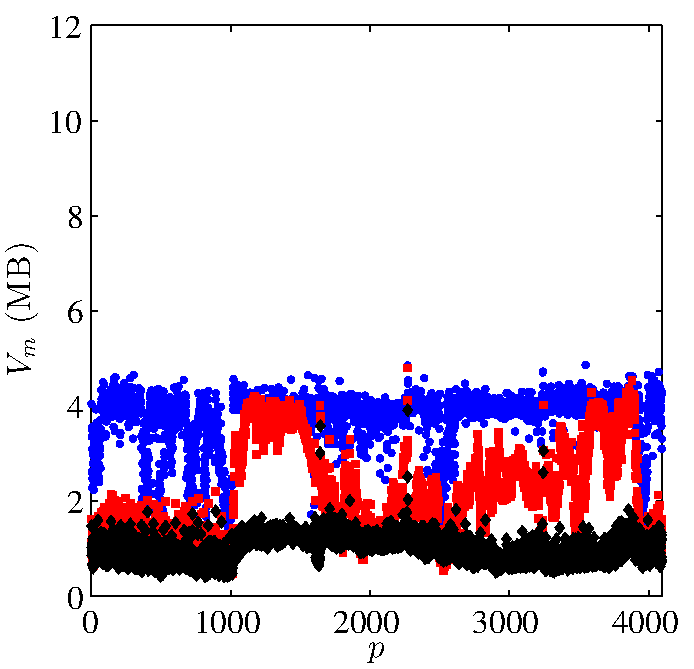
\includegraphics[width = 0.3 \textwidth] {figures/host_large_volume_last_4096.pdf}  \label{fig:communication_4096_vl}}		
	\end{center}
	\caption{Performance indicators of the first (top row) and last (bottom row) sub-iterations of the semi-Lagrangian algorithm for the level-set advection on 4096 processes with $\text{CFL} = 1$ (\drawdiamond{black}), $\text{CFL} = 10$ (\drawsquare{red}), and $\text{CFL} = 100$ (\drawcircle{blue}). Increasing the CFL number causes load imbalance during interpolation (a) and increases the communication volume (c). However, the CFL number does not seem to appreciably affect the number of messages sent by the processes (b). During the last semi-Lagrangian sub-iteration, the initial grid $G_0$ (cf.\ Algorithm \ref{alg:semi-lagrangian}) is very close to the final grid. As a result, the load imbalance is considerably improved (d). Curiously, however, the communication pattern does not seem to be change much between first and last sub-iterations (e,f).}
	\label{fig:communication_4096}
\end{figure}

\begin{table}[htbp]
	\centering
	\resizebox{\columnwidth}{!}{
	\begin{tabular}{|c|c|cccc|cccc|}
	\hline
	\multirow{2}{*}{CFL} & \multirow{2}{*}{Metric} & \multicolumn{4}{|c|}{First sub-iteration} & \multicolumn{4}{|c|}{Last sub-iteration} \\
	\cline{3-10}
											 & 												 & min & max & avg & stddev 					   & min & max & avg & stddev 						\\
	\hline
	\multirow{3}{*}{1}   & $N_p$        & 6.67E+04 & 1.59E+05 & 7.57E+04 & 4.86E+03 & 6.69E+04 & 1.55E+05 & 7.57E+04 & 4.73E+03 \\
										   & $N_m$ 			  & 18 			 & 387 		  & 47.55 	 & 31.72 		& 18 			 & 392 			& 47.55 	 & 31.19 		\\
										   & $V_m$ (MB)   & 4.01E-01 & 2.93E+00 & 7.25E-01 & 1.95E-01 & 4.13E-01 & 3.91E+00 & 9.68E-01 & 2.62E-01 \\
										   & $T_{\max}$ (s) & \multicolumn{4}{|c|}{6.96E-01}						& \multicolumn{4}{|c|}{3.67E-01}						\\
	\hline
	\multirow{3}{*}{10}  & $N_p$        & 5.56E+04 & 1.63E+05 & 7.57E+04 & 6.07E+03 & 6.65E+04 & 1.33E+05 & 7.57E+04 & 4.50E+03 \\
										   & $N_m$ 			  & 17 			 & 387 		  & 46.73 	 & 31.78 		& 19 			 & 393 			& 46.68 	 & 27.93 		\\
										   & $V_m$ (MB)   & 4.01E-01 & 3.06E+00 & 8.40E-01 & 2.21E-01 & 4.40E-01 & 4.80E+00 & 2.14E+00 & 9.88E-01 \\
											 & $T_{\max}$ (s) & \multicolumn{4}{|c|}{7.55E-01}						& \multicolumn{4}{|c|}{3.30E-01}						\\
	\hline
	\multirow{3}{*}{100} & $N_p$        & 8.28E+02 & 4.98E+05 & 7.57E+04 & 3.14E+04 & 6.30E+04 & 1.10E+05 & 7.57E+04 & 4.20E+03 \\
										   & $N_m$ 			  & 11 			 & 373 		  & 41.18 	 & 30.85 		& 16 			 & 357 			& 41.77 	 & 22.66 		\\
										   & $V_m$ (MB)   & 5.28E-01 & 1.01E+01 & 2.65E+00 & 9.24E-01 & 9.76E-01 & 4.86E+00 & 3.78E+00 & 5.69E-01 \\
											 & $T_{\max}$ (s) & \multicolumn{4}{|c|}{9.25E-01}						& \multicolumn{4}{|c|}{3.55E-01}						\\
	\hline
	\end{tabular}
	}
	\caption{Detailed load balancing and communication information for the advection test for $\text{CFL} = 1$, $\text{CFL} = 10$, and $\text{CFL} = 100$. Here $N_p$ is the number of interpolation points, $N_m = S + R$ is the number of sent ($S$) and received ($R$) messages, and $V_m$ is the total communication volume in megabytes (MB). Note how increasing the CFL number causes load imbalance and increases the communication volume while it does not affect the number of messages sent and received during a sub-iteration of the semi-Lagrangian step.}
	\label{tab:communication}
\end{table}

\subsection{Reinitialization} \label{section::scaling_reinitialization}

Finally we present the scaling results of our parallel reinitialization algorithm where we extensively make use of Algorithm \ref{alg:overlap} for overlapping the computations with the communications when computing spatial derivatives. Our test consists in computing the signed distance function to a collection of 100 spheres, whose radii and centers are chosen randomly. The test is performed on a small, level-8 Octree with about 21M and a larger, level-10 Octree with about 337M grid points. In both cases the forest is built on a $3\times3\times3$ macro-mesh. Figure \ref{fig:reinit} illustrates that our reinitialization algorithm, and in particular the overlapping strategy presented in Algorithm \ref{alg:overlap}, scales very well (cf.\ Table \ref{tab:scaling_reinit}). In general we expect similar scaling results for any local, finite-difference based calculations on Octrees that can efficiently utilize Algorithm \ref{alg:overlap}. 
\begin{figure}
\centering
\subfigure[]{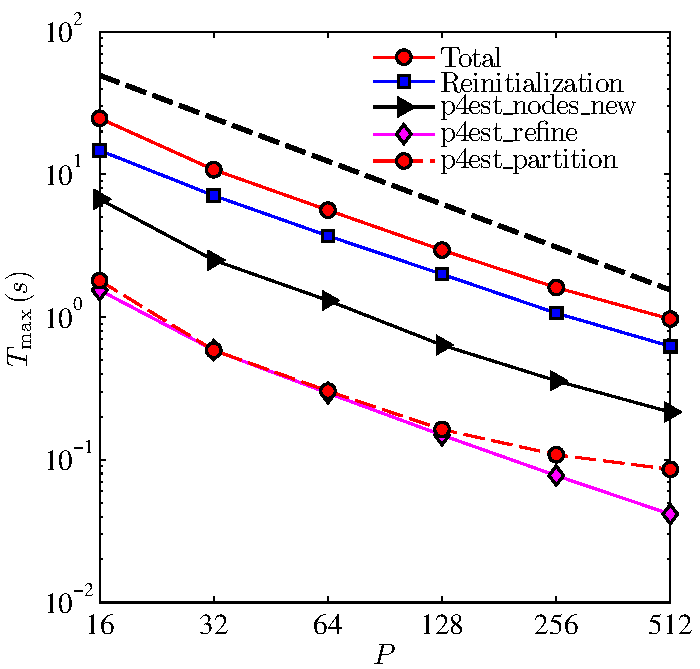
\includegraphics[width=0.48\textwidth]{figures/Reinit_Small.pdf}}
\subfigure[]{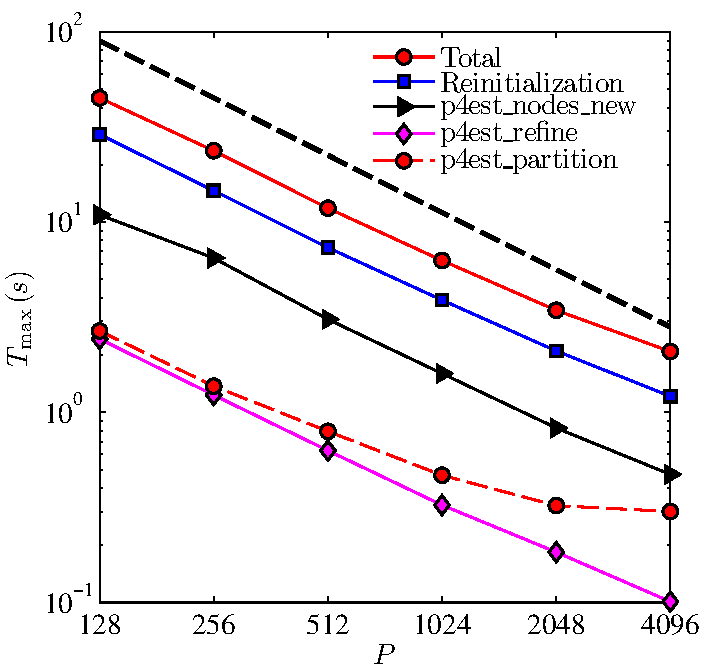
\includegraphics[width=0.48\textwidth]{figures/Reinit_Large.pdf}}
\caption{Scalability of the reinitialization test for a small (left) and large (right) Octree with roughly 21M and 337M grid points, respectively. The black dashed line represents ideal scaling. Excellent results are obtained in both cases, illustrating the scalability of the overlapping strategy (cf.\ Algorithm \ref{alg:overlap}).}
\label{fig:reinit}
\end{figure}

\begin{table}
\centering
	\begin{tabular}{|l|c|cccccc|}
	\hline
	\multirow{2}{*}{Small Test} & $P$ & 16      & 32      & 64      & 128     & 256    & 512 \\ 	                            
	                            & $e$ & $100\%$ & $115\%$ & $110\%$ & $105\%$ & $96\%$ & $80\%$ \\
	\hline
	\multirow{2}{*}{Large Test} & $P$ & 128     & 256     & 512     & 1024    & 2048   & 4096 \\ 	                            
	                            & $e$ & $100\%$ & $95\%$ & $95\%$ & $89\%$ & $82\%$ & $67\%$ \\
	\hline
	\end{tabular}
	\caption{Parallel efficiency of the total runtime for the reinitialization test based on the lowest number of processes for each test.}
	\label{tab:scaling_reinit}
\end{table}

% %!TEX root = draft.tex
\section{Application to the Stefan problem} \label{sec:application}

\subsection{Presentation of the problem}

In this section we apply our approach to the study of the phase transition of a liquid melt to a solid crystaline structure. In the case of a single component melt, and in the absence of convection, the process is dominated by diffusion and can be modeled as a Stefan problem. We decompose the computational domain $\Omega$ into two subdomains $\Omega_l$ and $\Omega_s$, separated by an interface $\Gamma$. The Stefan problem describes the evolution of the temperature $T$, decomposed into $T_s$ in the solid phase $\Omega_s$ and $T_l$ in the liquid phase $\Omega_l$, as
\begin{align}
\pd{T_l}{t} & = D_l \Delta T_l \quad \mathrm{in} ~~ \Omega_l, \label{eq:stefan_heat_equation_l} \\
\pd{T_s}{t} & = D_s \Delta T_s \quad \mathrm{in} ~~ \Omega_s. \label{eq:stefan_heat_equation_s}
\end{align}
The diffusion constants $D_l$ and $D_s$ can be discontinuous across the interface. We prescribe homogeneous Neumann boundary conditions on the edge of the computational domain, $\nabla T \cdot \underline{\mathbf{n}}\vert_{\partial \Omega}=0$. At the interface between the solid and the liquid phases, the temperature is given by the Gibbs-Tompson boundary condition \cite{Alexiades;Solomon;Wilson:88:The-formation-of-a-s, Alexiades;Solomon:93:Mathematical-Modelin}:
\begin{equation} \label{eq:stefan_gibbs_tompson}
T_s = T_l = T_{\Gamma} = -\epsilon_c \kappa - \epsilon_v (\underline{\mathbf{u}} \cdot \underline{\mathbf{n}}),
\end{equation}
where $\kappa$ is the local interface curvature, $\underline{\mbf{u}}$ is the velocity of the interface, $\underline{\mathbf{n}}$ is the outward normal to the solidification front and $\epsilon_c$ and $\epsilon_v$ are the surface tension and kinetic undercooling coefficients. The interface velocity $\underline{\mbf{u}}$ is defined from the jump in the heat flux at the interface,
\begin{equation} \label{eq:stefan_velocity}
(\underline{\mathbf{u}} \cdot \underline{\mathbf{n}}) = - \left[ D_l \pd{T_l}{\underline{\mathbf{n}}} - D_s \pd{T_s}{\underline{\mathbf{n}}} \right].
\end{equation}
We choose to use an adaptive time step with a $\text{CFL} = 5$, i.e.
\begin{equation} \label{eq:stefan_dt}
\Delta t = 5 ~ \Delta x_{min} ~ \min(1,1/\max \lVert \underline{\mathbf{u}} \rVert),
\end{equation}
where $\Delta x_{min}$ is the size of the smallest cell of the forest. The general procedure to solve the Stefan problem is presented in Algorithm \ref{alg:stefan} and we refer the interested reader to \cite{Chen;Min;Gibou:09:A-numerical-scheme-f} for the details of implementation. In implementing the numerical solver, we make use of the popular \texttt{PETSc}
\cite{Balay;Abhyankar;Adams;etal:14:PETSc-Web-page} library for linear algebra and its parallel primitives, such as parallel ghosted vector and scatter/gather operations, which simplifies the implementation.


\begin{algorithm}[htbp]
\caption{$\texttt{General procedure for solving the Stefan problem}$}
\begin{algorithmic}[1]
\State Initialize the forest and $\phi$ given the initial geometry.
\State Initialize $T_s$ in $\Omega^+$ and $T_l$ in $\Omega^-$.
\State Reinitialize $\phi$ and compute the local interface curvature $\kappa$.
\State Compute $T^{n+1}_l$ and $T^{n+1}_s$ by solving the heat equations \eqref{eq:stefan_heat_equation_l} and \eqref{eq:stefan_heat_equation_s}.
\State Extrapolate $T^{n+1}_s$ from $\Omega^+$ to $\Omega^-$ and $T^{n+1}_l$ from $\Omega^-$ to $\Omega^+$.
\State Compute the velocity field $\underline{\mathbf{u}}$ according to \eqref{eq:stefan_velocity}.
\State Compute the time step dt following \eqref{eq:stefan_dt}.
\State Evolve the interface and construct the new forest using the Semi-Lagrangian procedure.
\State Interpolate $T^{n+1}_s$ and $T^{n+1}_l$ from the old forest to the new forest.
\State Go to 3 with n=n+1.
\end{algorithmic}
\label{alg:stefan}
\end{algorithm}

\subsection{Scalability}

The implementation of the Stefan problem relies on the components described in the previous sections, and it is therefore a good synthesis of the performance of the various algorithms. We monitored the performance of the code over five time iterations, as presented in Algorithm \ref{alg:stefan}, for two different maximum resolutions. In both cases, the forest is built on a $20\times20\times20$ macro-mesh. The maximum tree resolution for the small test is 9, leading to approximately 7M grid points, and the maximum resolution for the large test is 11, corresponding to 105M grid points. The results are presented in figure \ref{fig:stefan_scaling}, where ``\verb|Solution_Extension|'' refers to extrapolation procedure (see Algorithm \ref{alg:stefan} step 5). As expected from the results obtained for each component in the previous sections, our implementation of the Stefan problem exhibits very satisfactory scaling (cf.\ Table \ref{tab:scaling_stefan}).

\begin{figure}
\centering
\subfigure[]{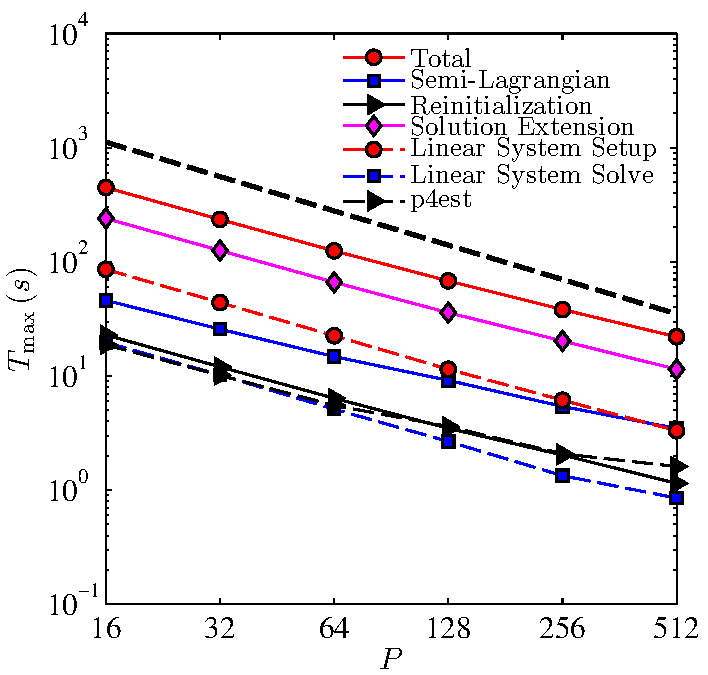
\includegraphics[width=0.48\textwidth]{figures/Stefan_small.pdf}}
\subfigure[]{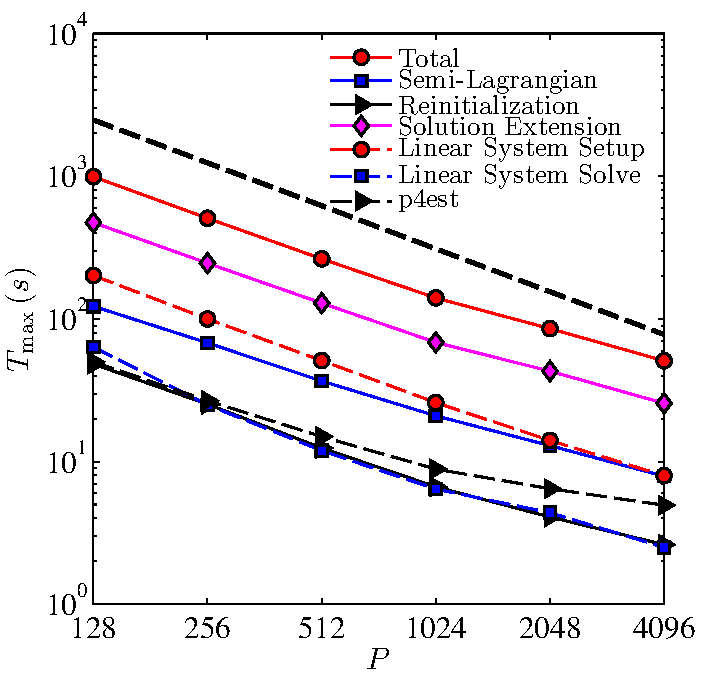
\includegraphics[width=0.48\textwidth]{figures/Stefan_large.pdf}}
\caption{Scalability of the Stefan problem for small (left) and large (right) Octrees with roughly 7M and 105M grid points, respectively. The solid dashed line represents perfect scaling. As expected from the scalability analysis of the individual components, we observe excellent results, illustrating the potential of our algorithms.}
\label{fig:stefan_scaling}
\end{figure}

\begin{table}
\centering
	\begin{tabular}{|l|c|cccccc|}
	\hline
	\multirow{2}{*}{Small Test} & $P$ & 16      & 32      & 64      & 128     & 256    & 512 \\ 	                            
	                            & $e$ & $100\%$ & $95\%$  & $90\%$  & $82\%$  & $73\%$ & $64\%$ \\
	\hline
	\multirow{2}{*}{Large Test} & $P$ & 128     & 256     & 512     & 1024    & 2048   & 4096 \\ 	                            
	                            & $e$ & $100\%$ & $98\%$  & $94\%$  & $89\%$  & $73\%$ & $61\%$ \\
	\hline
	\end{tabular}
	\caption{Parallel efficiency of the total runtime for the Stefan test based on the lowest number of processes for each test.}
	\label{tab:scaling_stefan} 
\end{table}

\subsection{Numerical experiments}
We now present the results from a large simulation of the Stefan problem on a $20\times20\times20$ macro-mesh and with level-10 Octrees. The Gibbs-Tompson anisotropy undercooling coefficients in equation \eqref{eq:stefan_gibbs_tompson} are defined as
\begin{align*}
\epsilon_c & = \left[ \epsilon_1 \left( 1+\alpha_1 \cos(3\theta_1) \right) + \epsilon_2 \left( 1+\alpha_2 \cos(3\theta_2) \right) \right] \kappa,\\
\epsilon_v & = 0,
\end{align*}
with $\theta_1$ the angle between the normal to the interface $\underline{\mathbf{n}}$ and the x-axis in the $(x,y)$ plane and $\theta_2$ the angle between $\underline{\mathbf{n}}$ and the x-axis in the $(x,z)$ plane. The coefficients
\begin{align*}
\epsilon_1 & = 2~(\sin(x)+\cos(y)+2)\cdot10^{-6}, & \epsilon_2 & = 2~(\sin(x)+\cos(z)+2)\cdot10^{-6}, \\
\alpha_1 & = \frac{1}{4}(\cos(x)+\sin(y)+2), & \alpha_2 & = \frac{1}{4}(\cos(x)+\sin(z)+2),
\end{align*}
are used to enforce a variety of crystal shapes. The computation is initialized with twenty spherical seeds of radius $1.5 \cdot 10^{-3}$ placed randomly in the domain. We take the diffusion coefficients $D_s=D_l=1$ and set the initial temperatures $T^0_l=-0.25$ and $T^0_s=0$.

The simulation was ran on $256$ MPI processes for $6$ hours and $30$ minutes, resulting in $396$ time iterations. Visualizations of the final iteration are presented in figures \ref{fig:stefan_grid} and \ref{fig:stefan_evolution}. The final iteration of the simulation consisted of $167$M grid points whereas a uniform grid with the equivalent finest resolution would lead to $8.59\cdot10^{12}$ grid points, i.e. over eight trillion grid points. Our simulation used only $0.002\%$ of the number of grid points needed for the same simulation on a uniform grid. This application demonstrates the ability of our approach to resolve small scale details, while accounting for long range interactions.

\begin{figure}[ht!]
\begin{center}
\subfigure[]{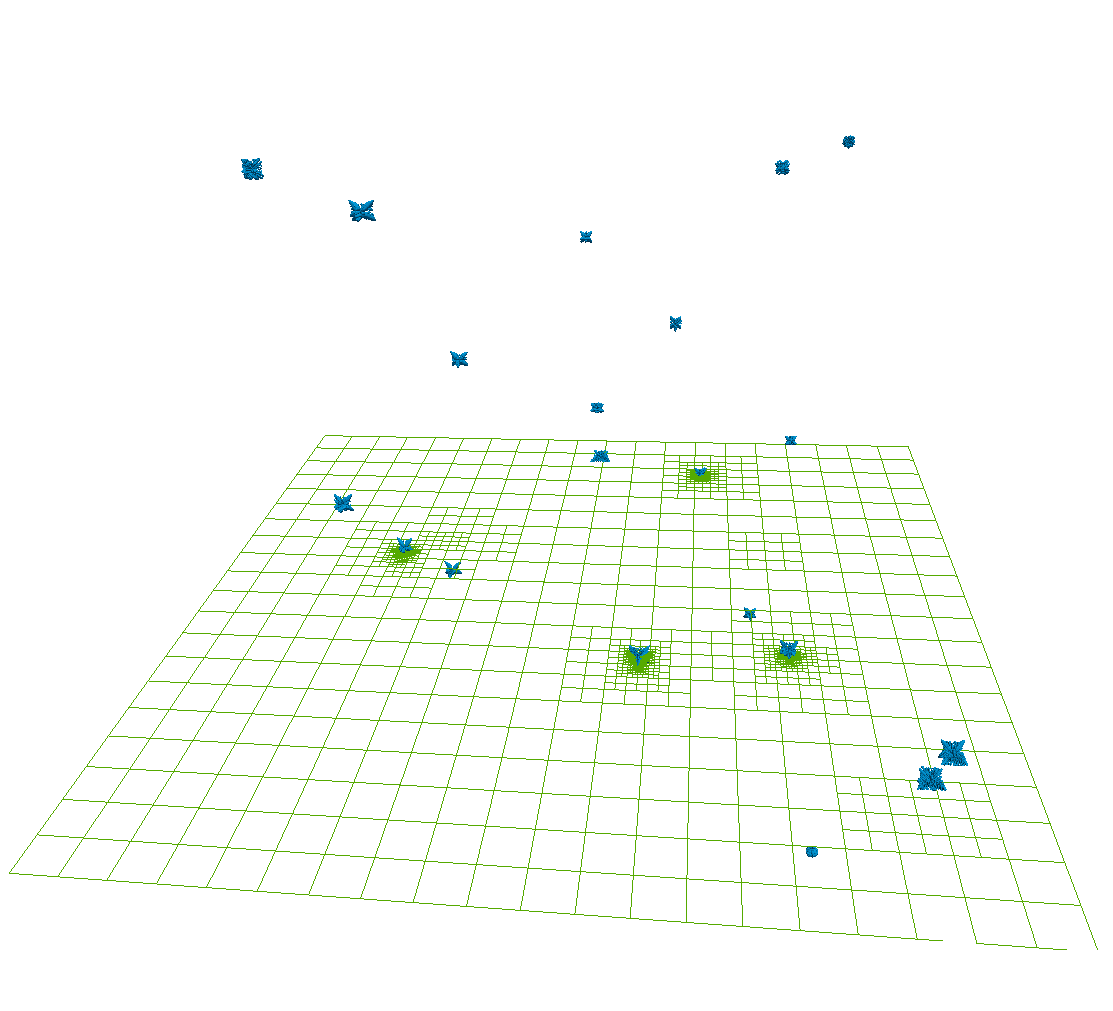
\includegraphics[width=0.45\textwidth]{figures/stefan_grid_overview.png}}
\subfigure[]{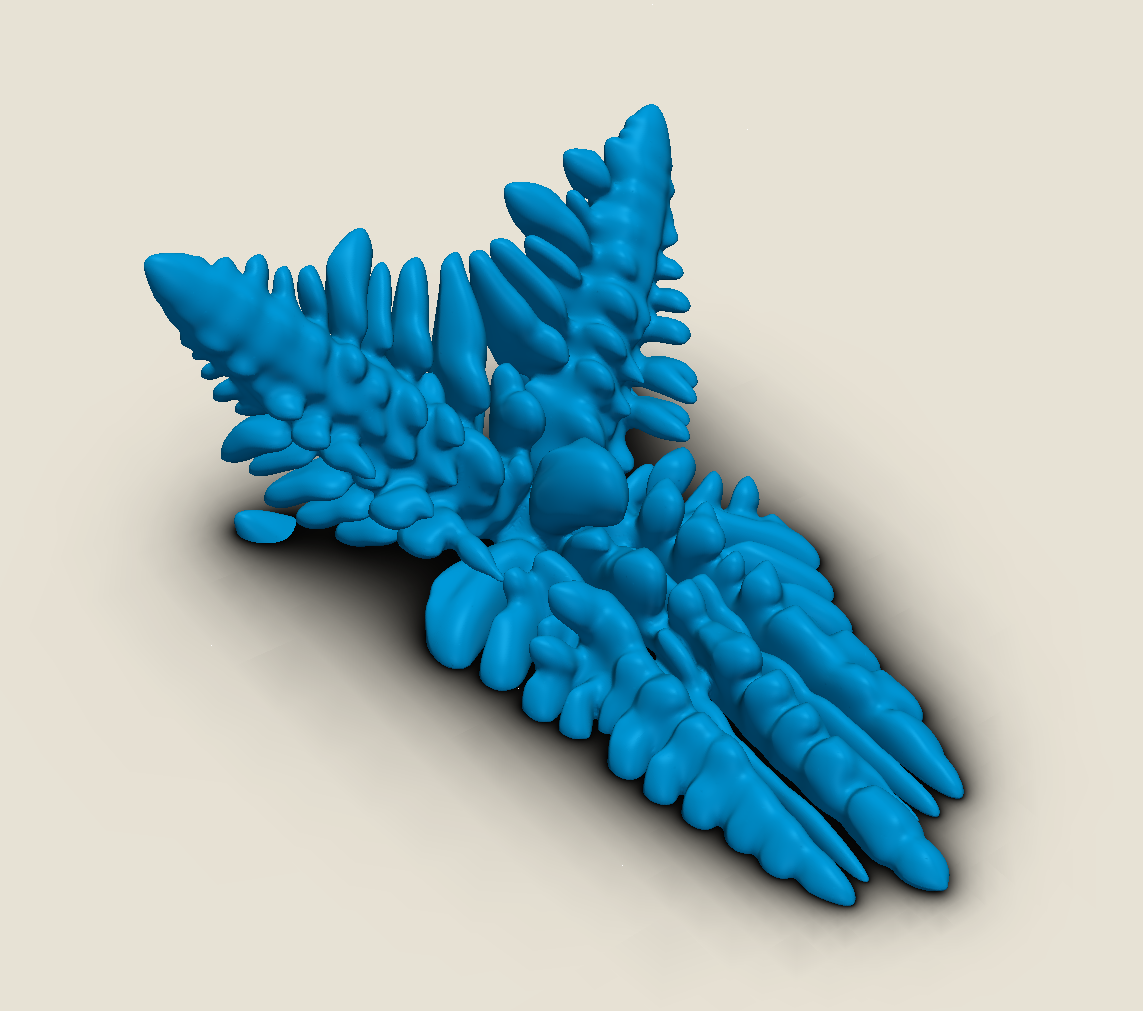
\includegraphics[width=0.45\textwidth]{figures/stefan_temperature.png}}
\subfigure[]{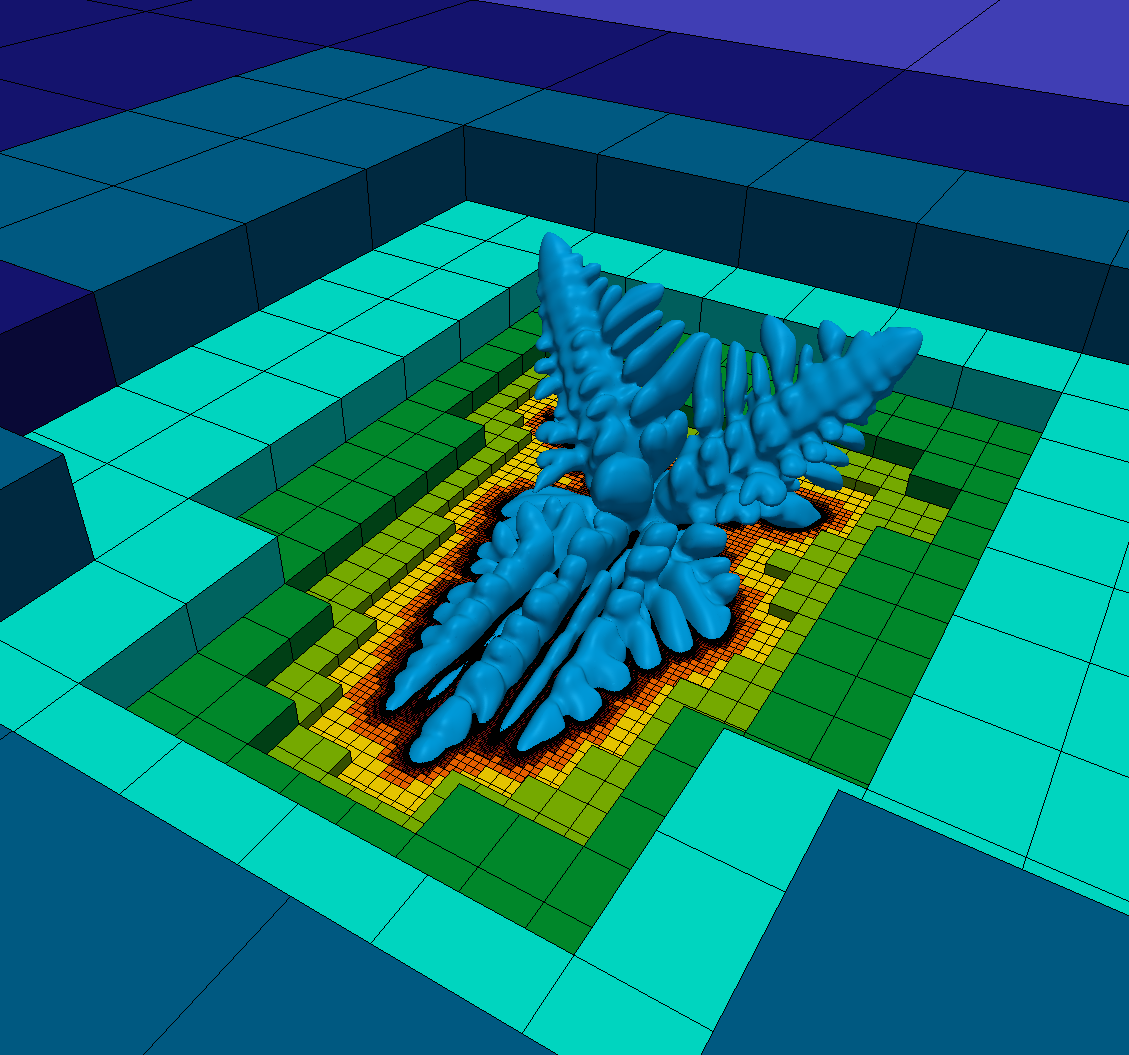
\includegraphics[width=0.45\textwidth]{figures/stefan_grid.png}}
\subfigure[]{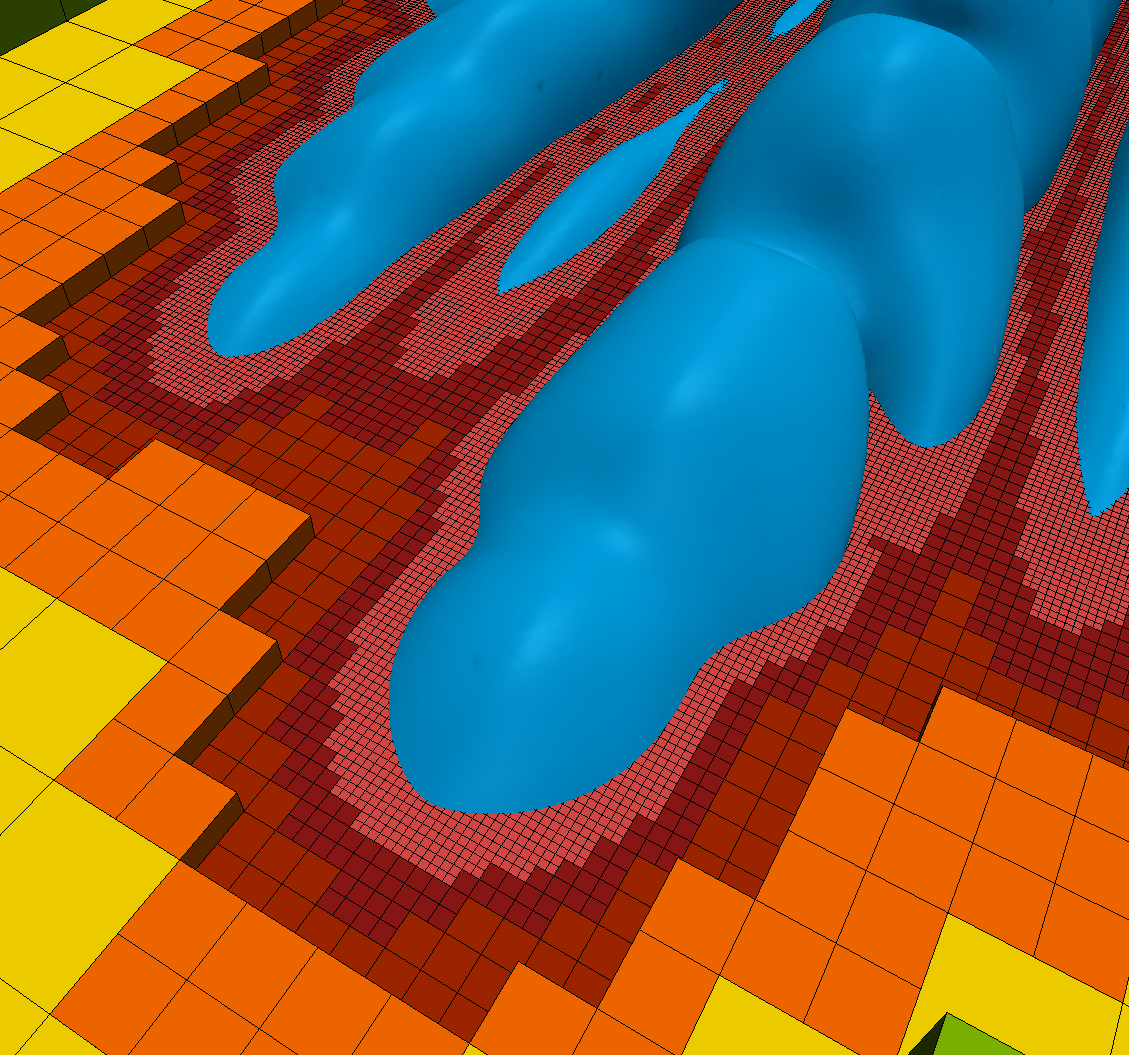
\includegraphics[width=0.45\textwidth]{figures/stefan_grid_zoom.png}}
\caption{Visualization of the computational mesh (a, c, d) and the temperature field (b) for the Stefan problem simulation.} \label{fig:stefan_grid}
\end{center}
\end{figure}

%\begin{figure}[ht!]
%\begin{center}
%\subfigure[]{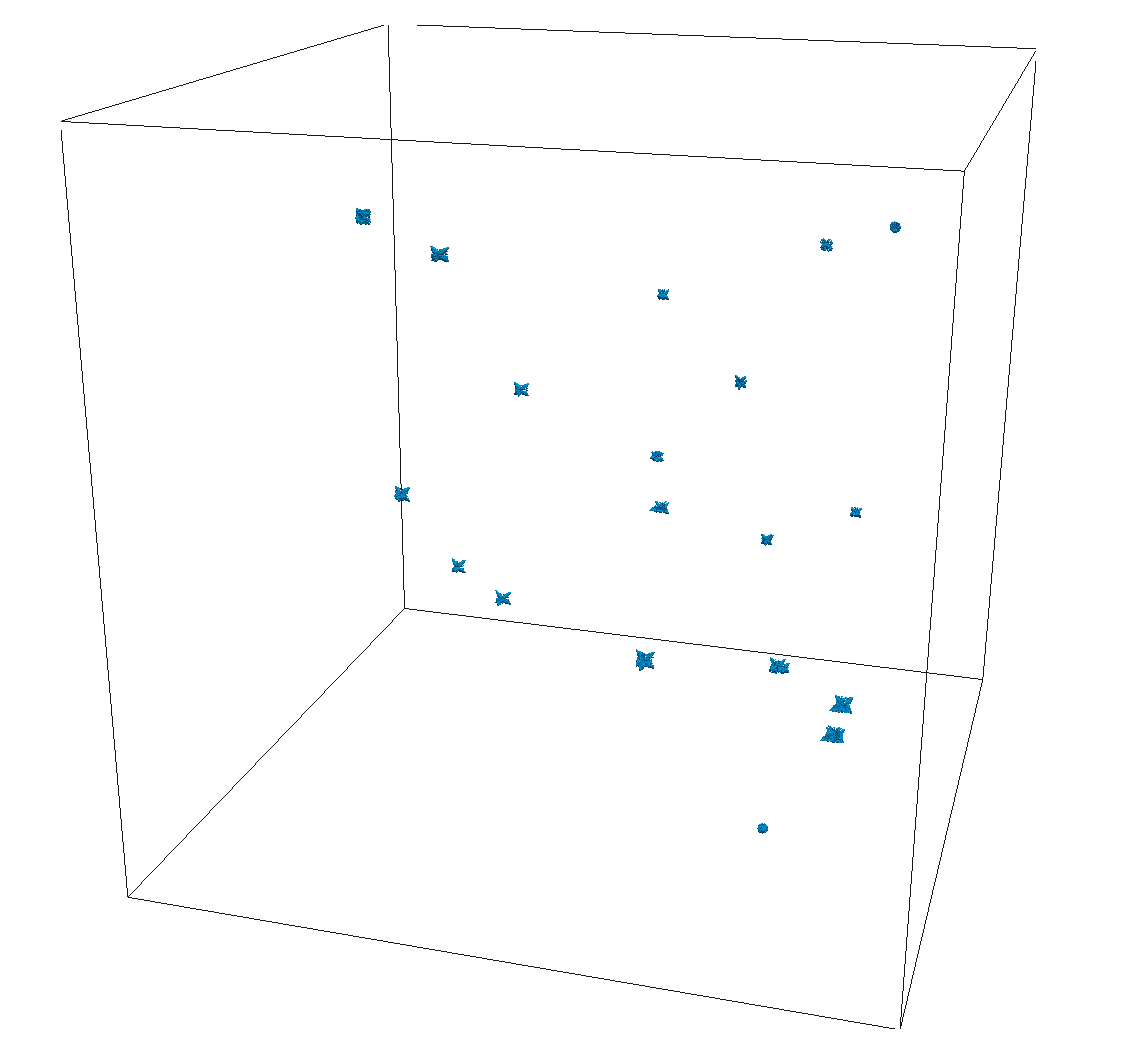
\includegraphics[width=0.45\textwidth]{figures/stefan_crystal_1.png}}
%\subfigure[]{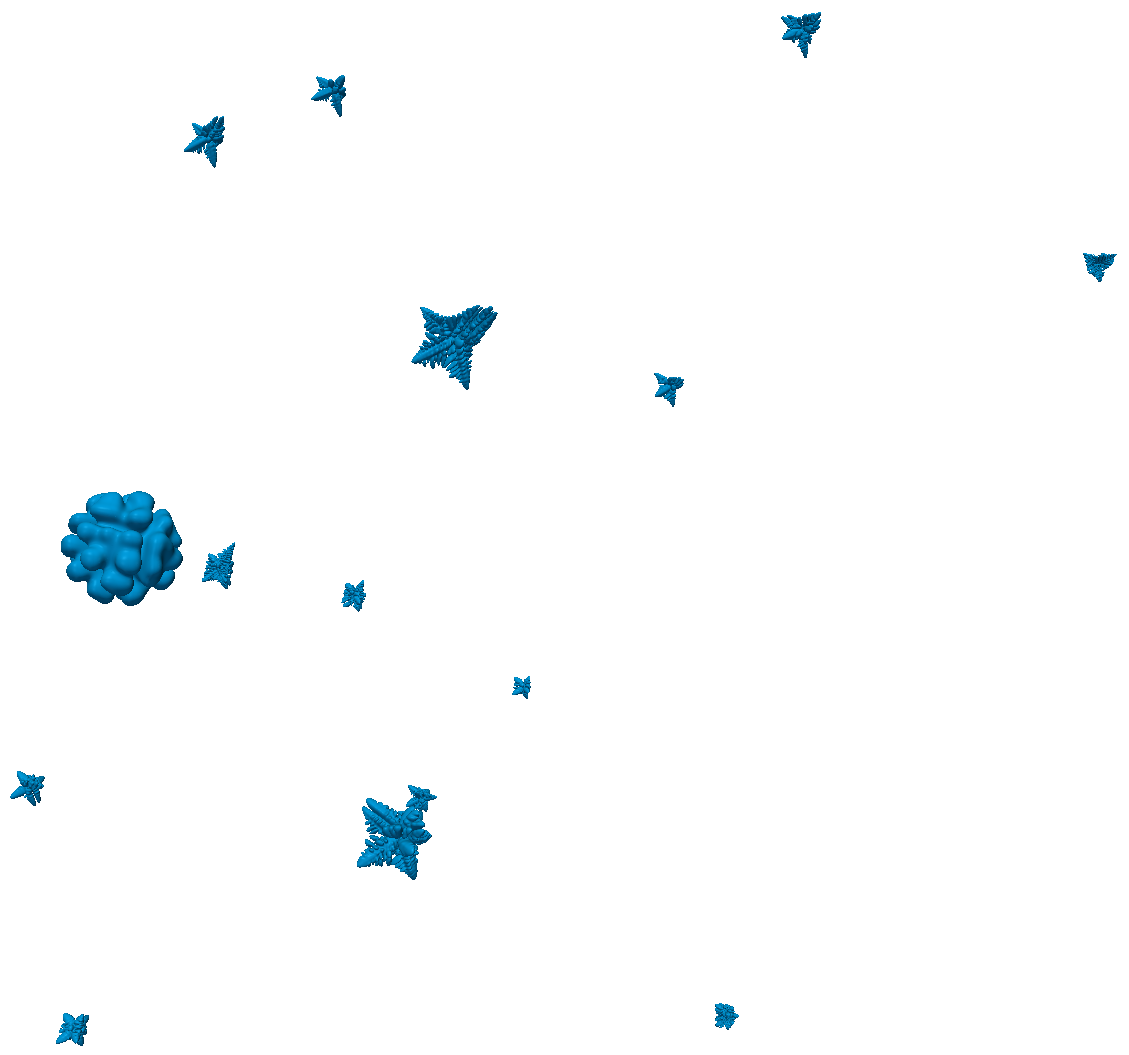
\includegraphics[width=0.45\textwidth]{figures/stefan_crystal_2.png}}
%\subfigure[]{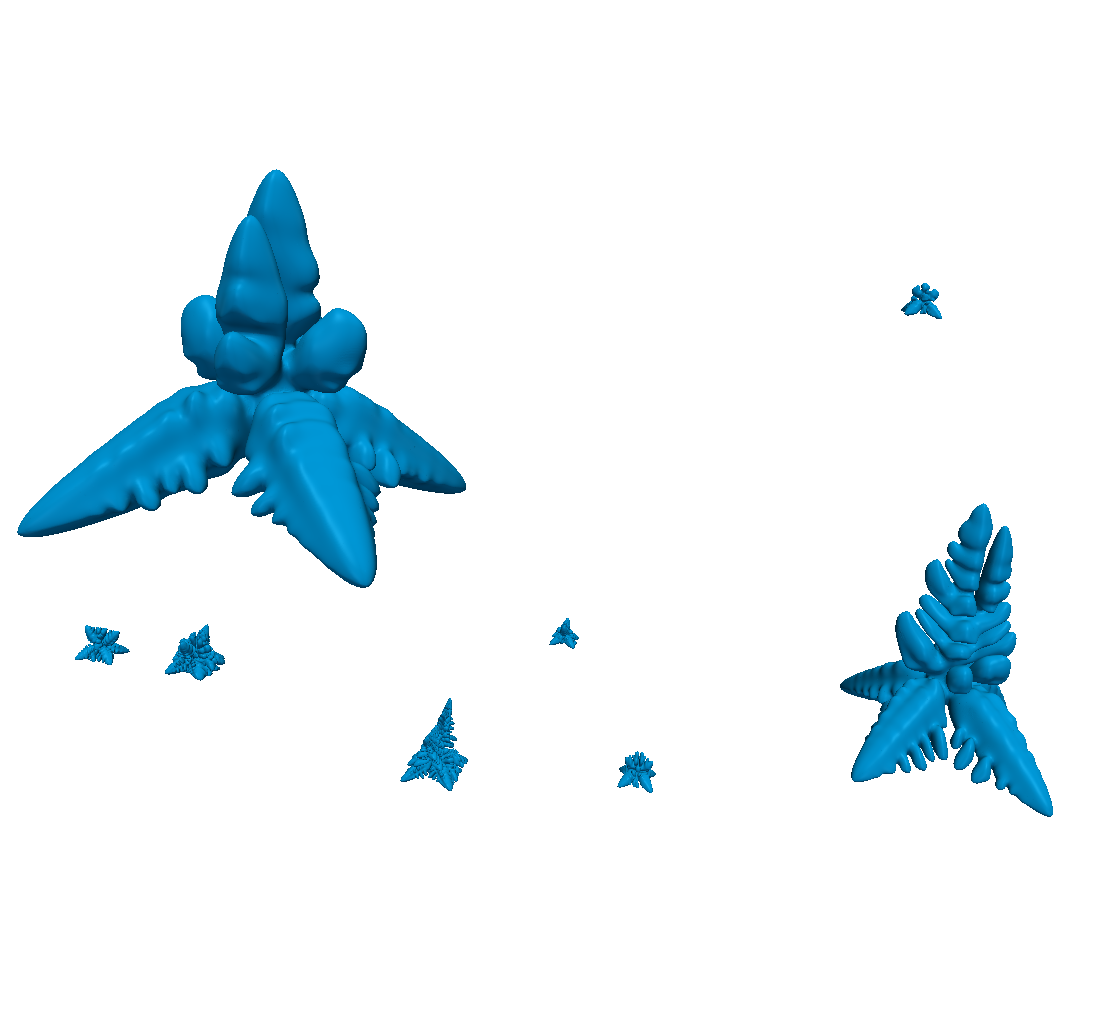
\includegraphics[width=0.45\textwidth]{figures/stefan_crystal_4.png}}
%\subfigure[]{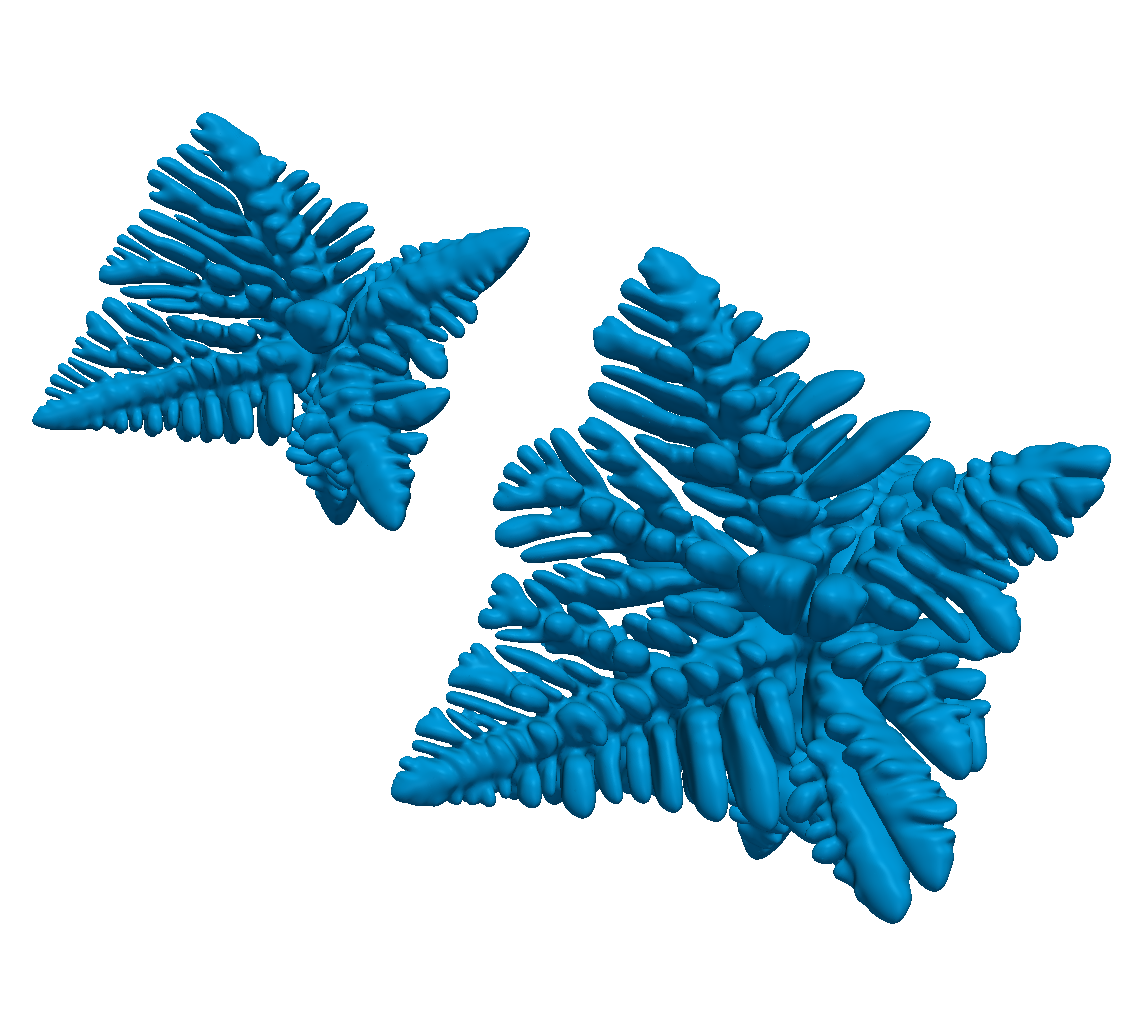
\includegraphics[width=0.45\textwidth]{figures/stefan_crystal_3.png}}
%\caption{Representation of the computational domain (a) as well as various developped crystal structures obtained from solving the Stefan problem simulation (b,c,d).} \label{fig:stefan_crystals}
%\end{center}
%\end{figure}

\begin{figure}[ht!]
\begin{center}
\subfigure{
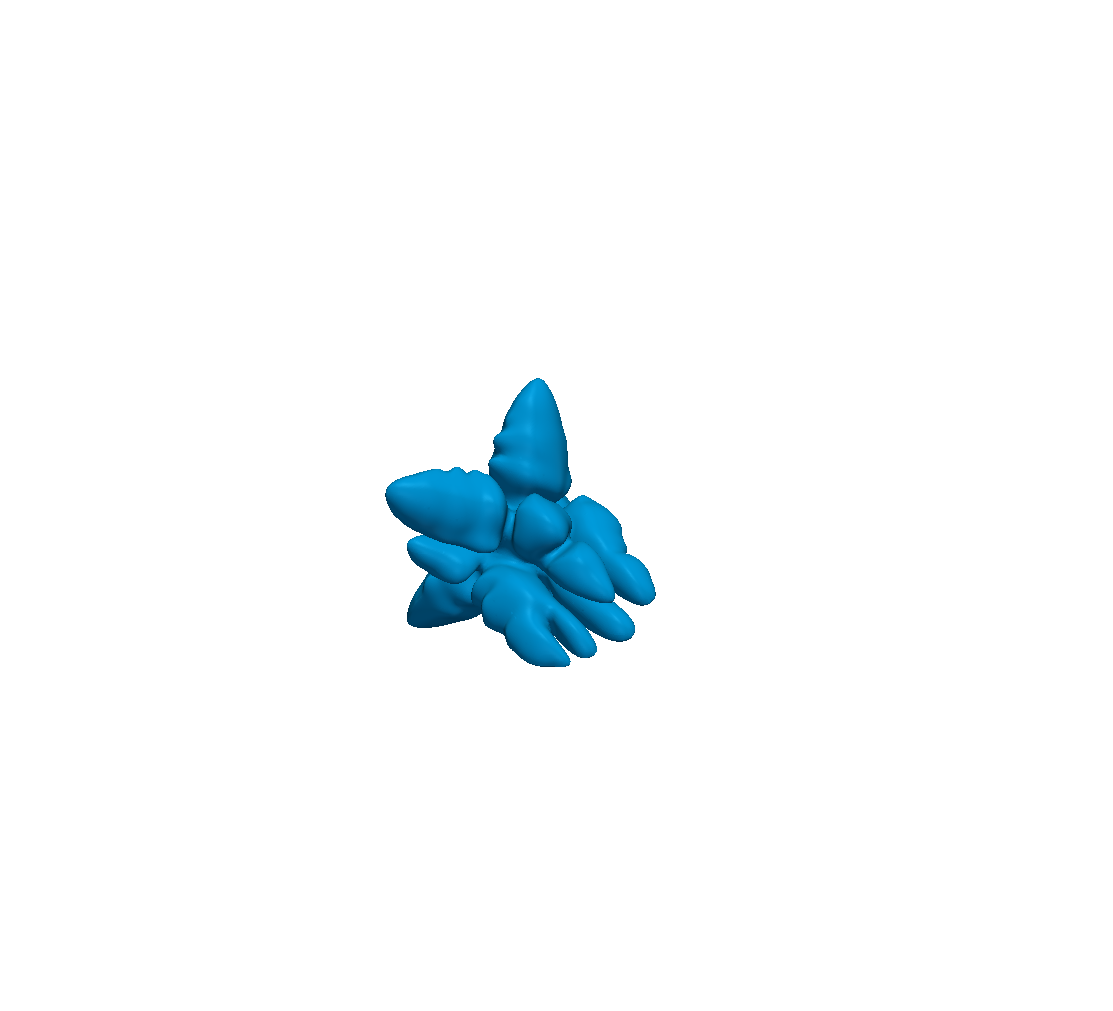
\includegraphics[width=.24\textwidth]{stefan/nb2_iter19.png}
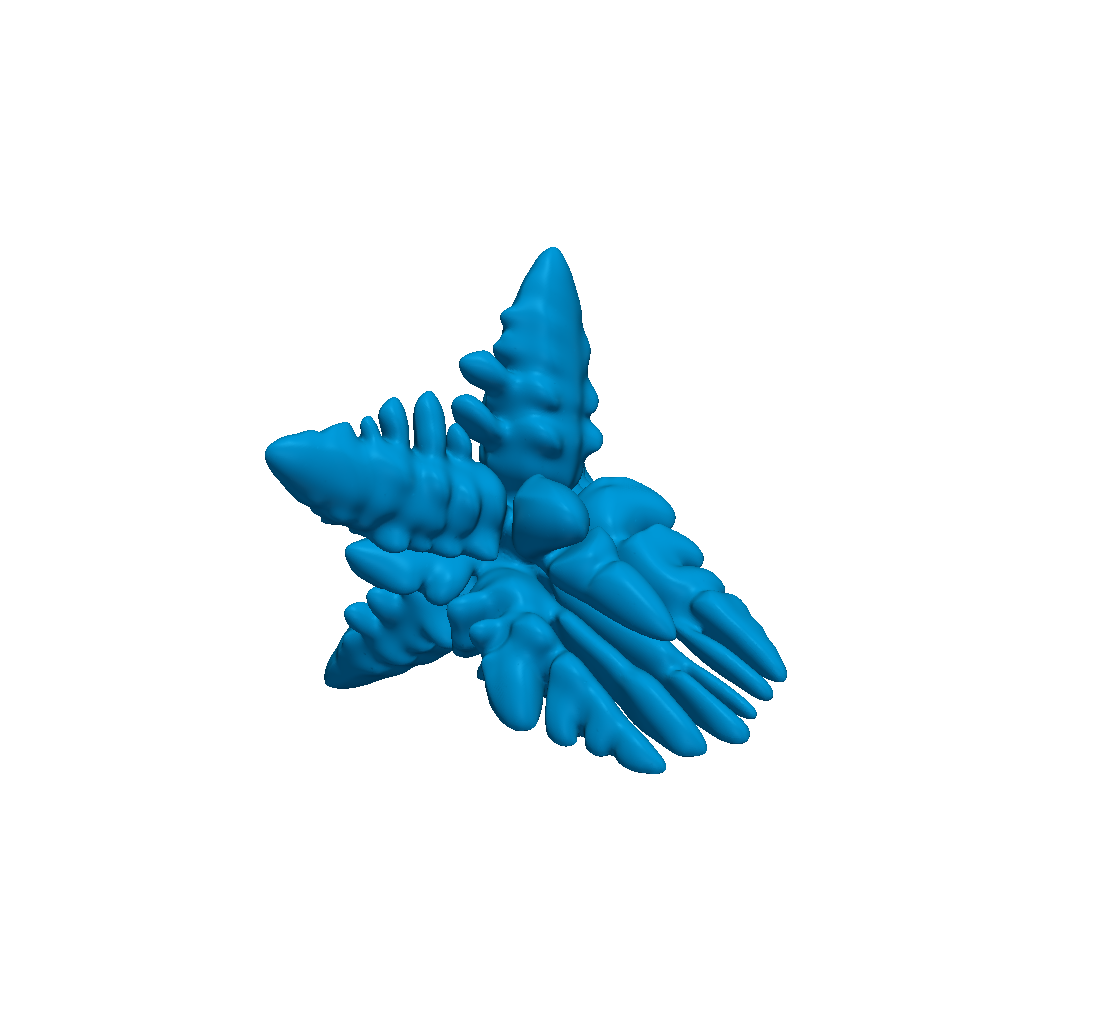
\includegraphics[width=.24\textwidth]{stefan/nb2_iter39.png}
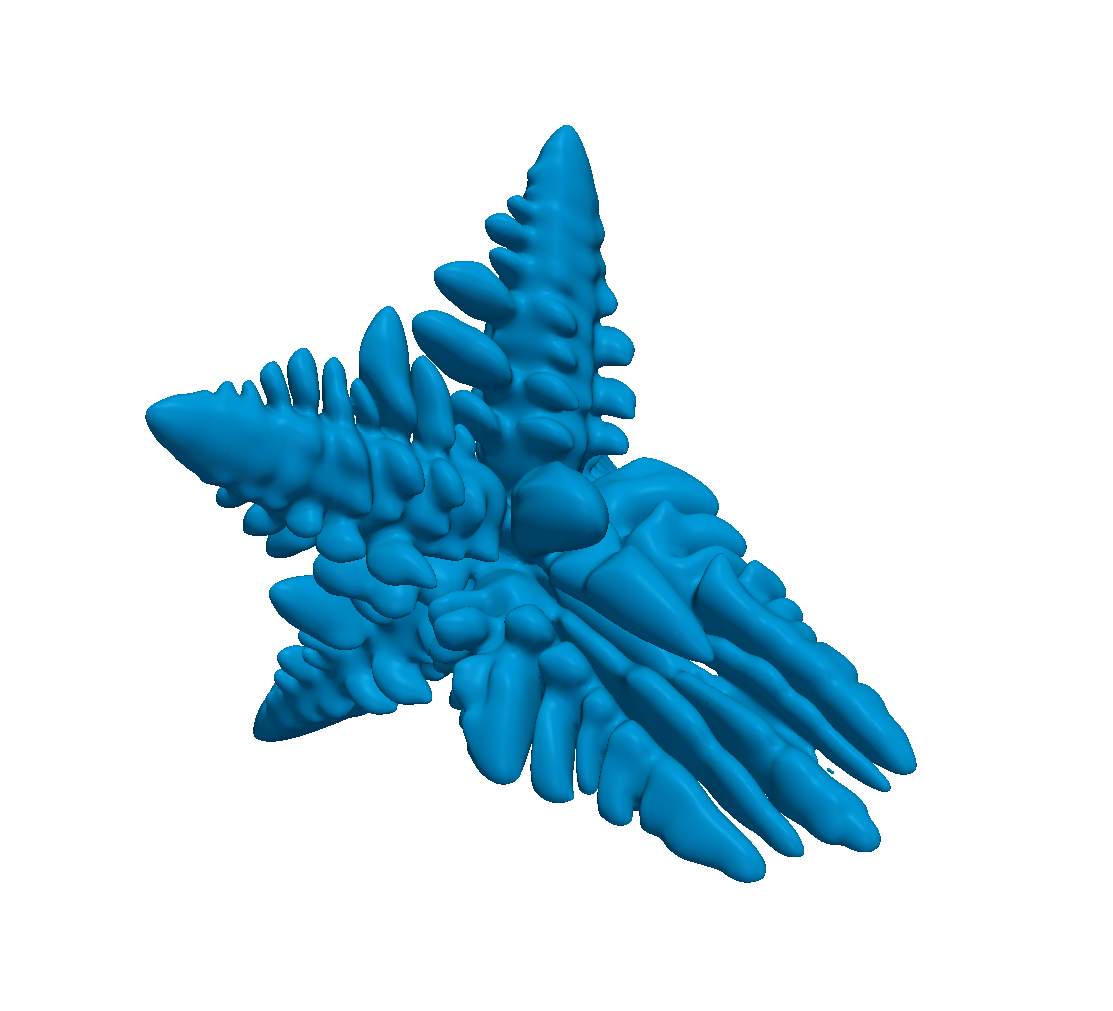
\includegraphics[width=.24\textwidth]{stefan/nb2_iter59.png}
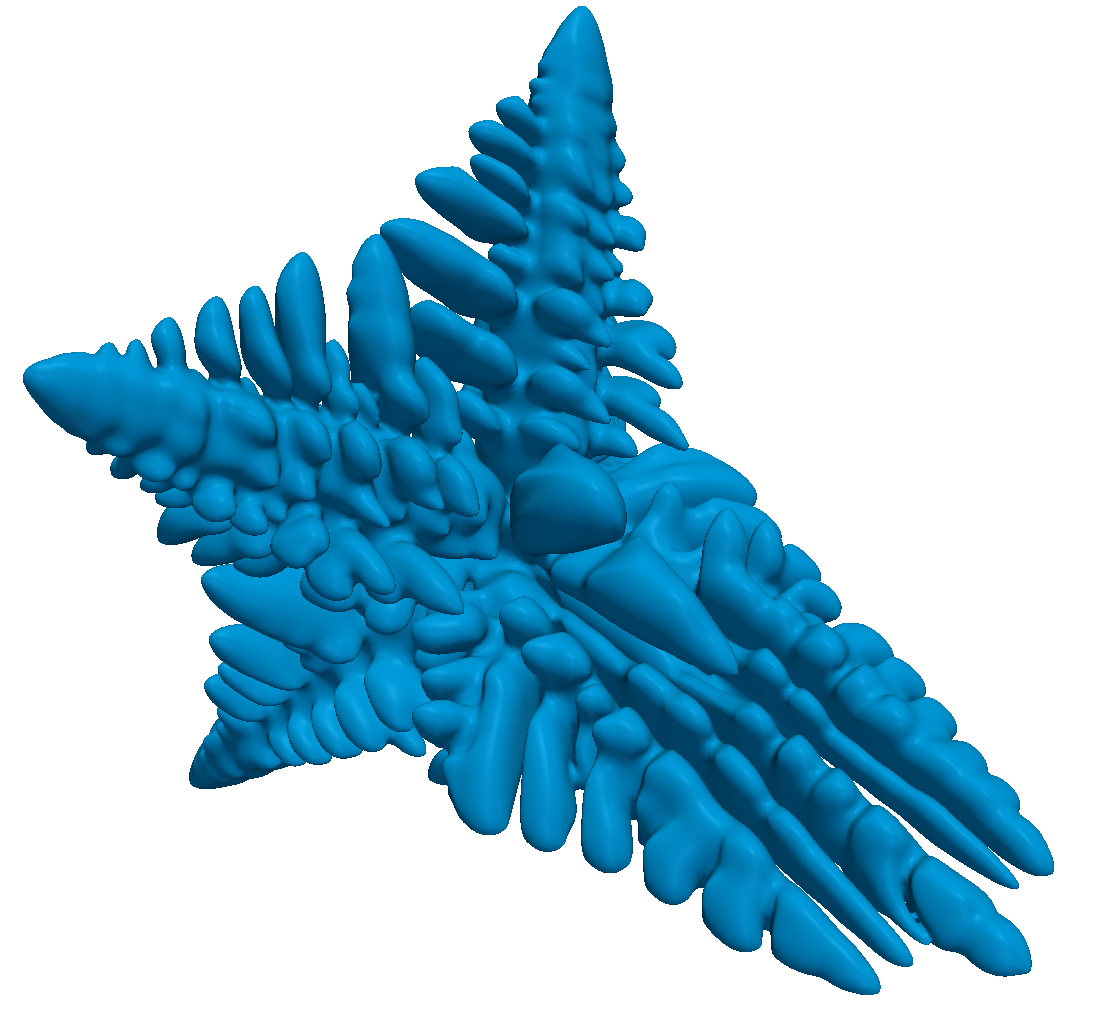
\includegraphics[width=.24\textwidth]{stefan/nb2_iter79.png}
}
\subfigure{
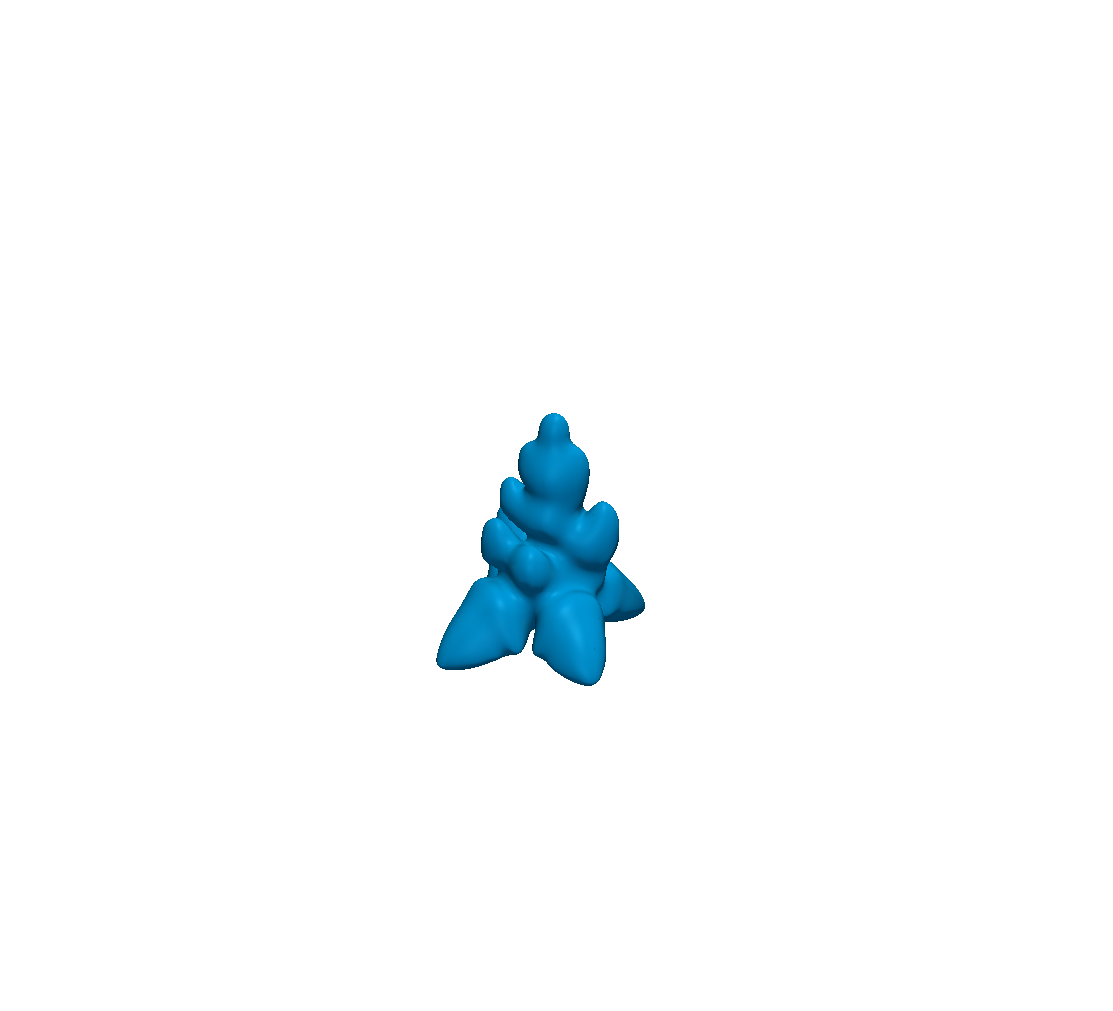
\includegraphics[width=.24\textwidth]{stefan/nb5_iter19.png}
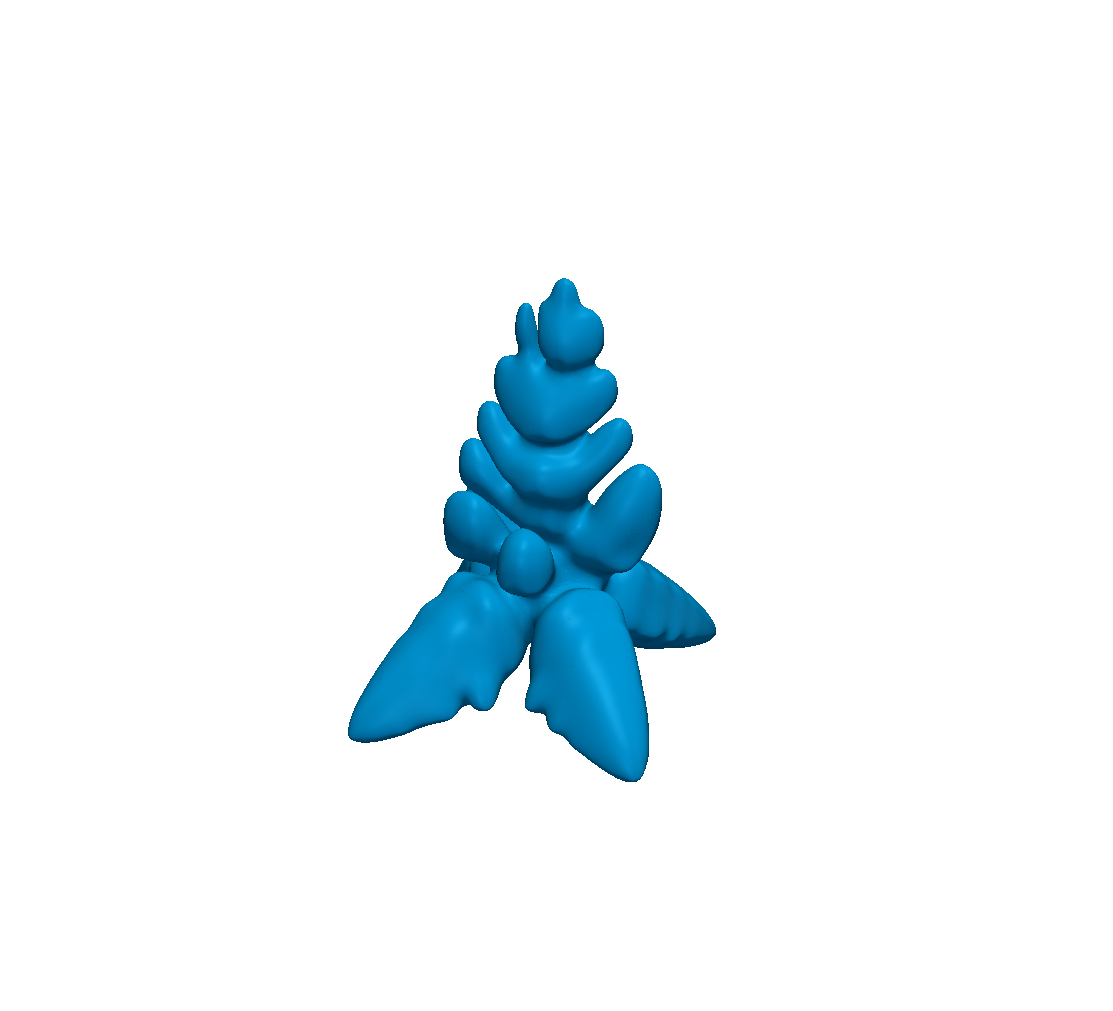
\includegraphics[width=.24\textwidth]{stefan/nb5_iter39.png}
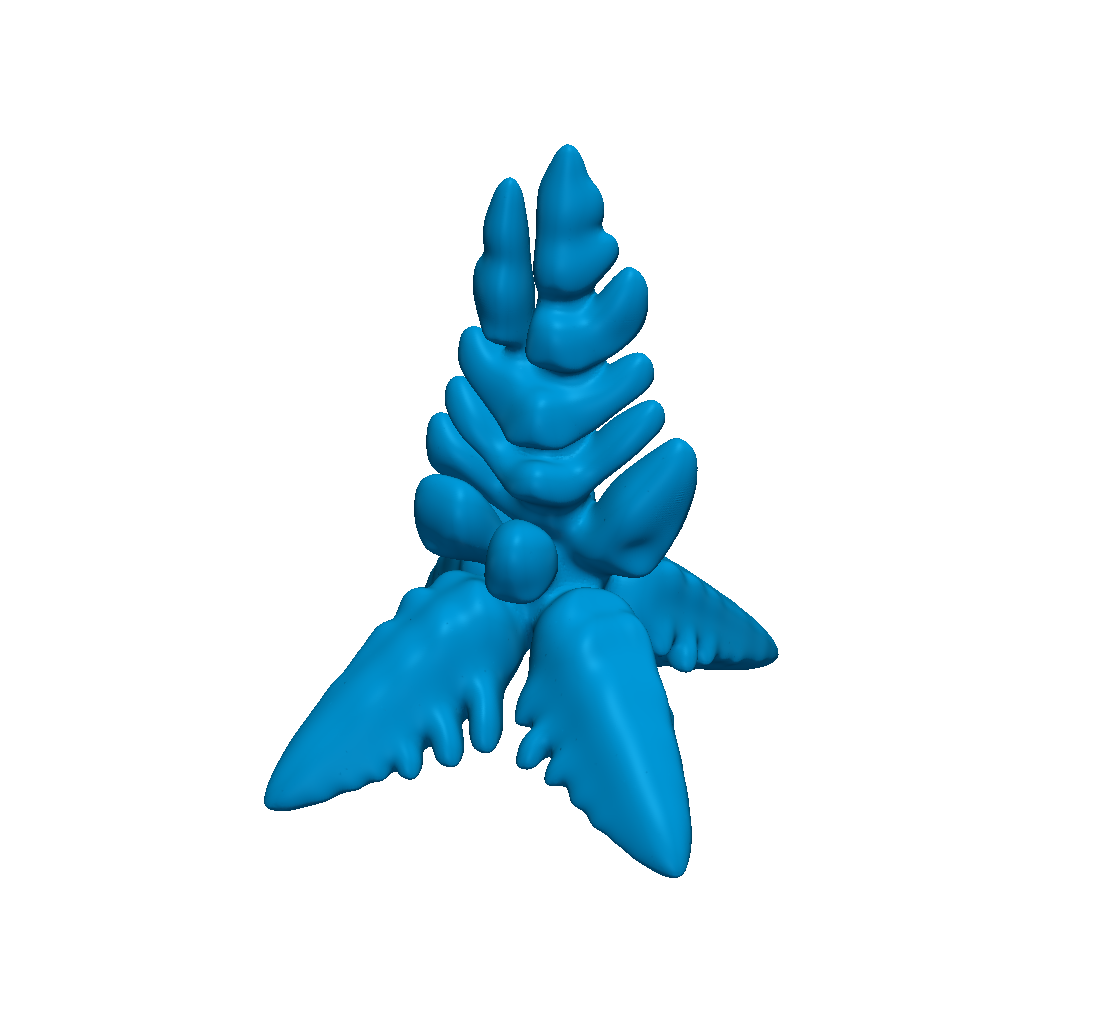
\includegraphics[width=.24\textwidth]{stefan/nb5_iter59.png}
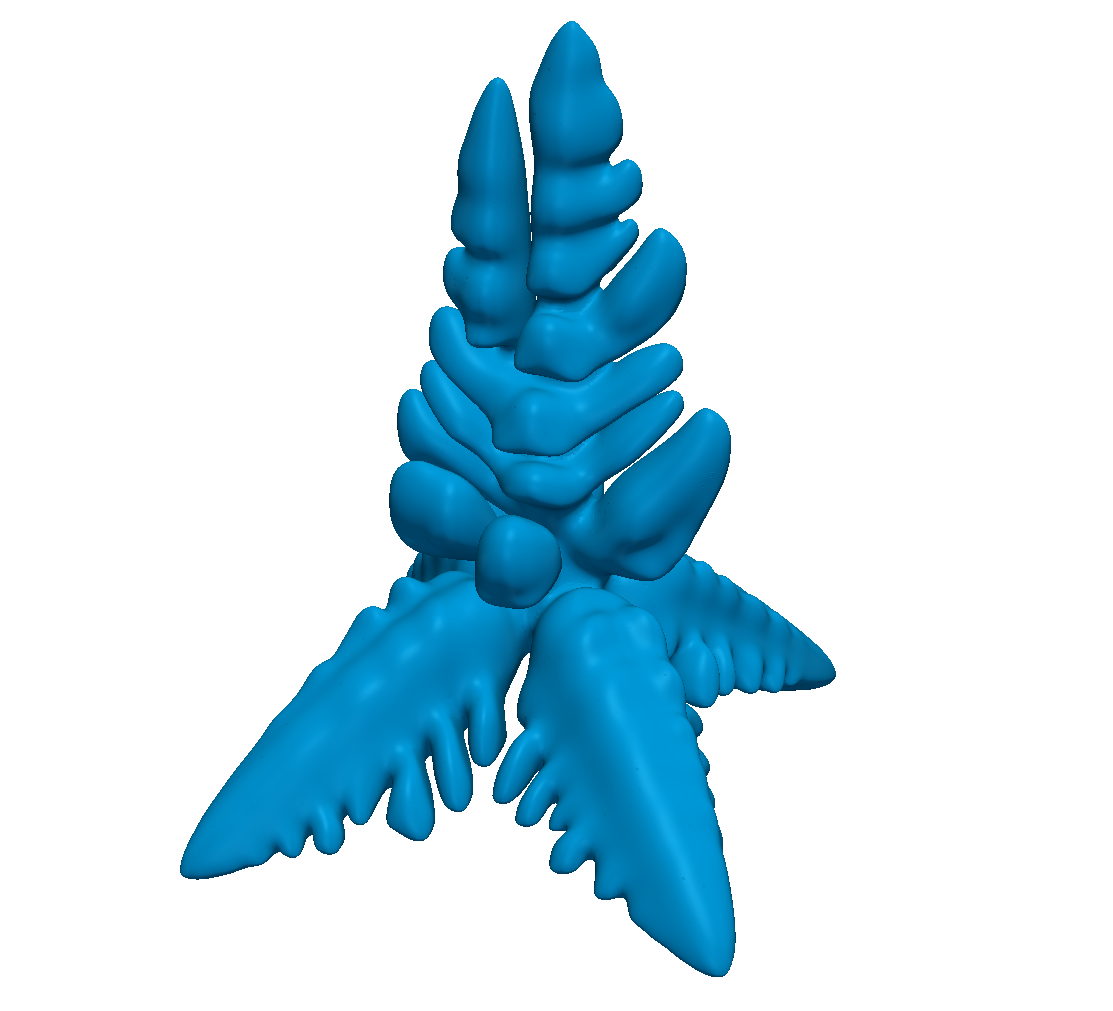
\includegraphics[width=.24\textwidth]{stefan/nb5_iter79.png}
}
\subfigure{
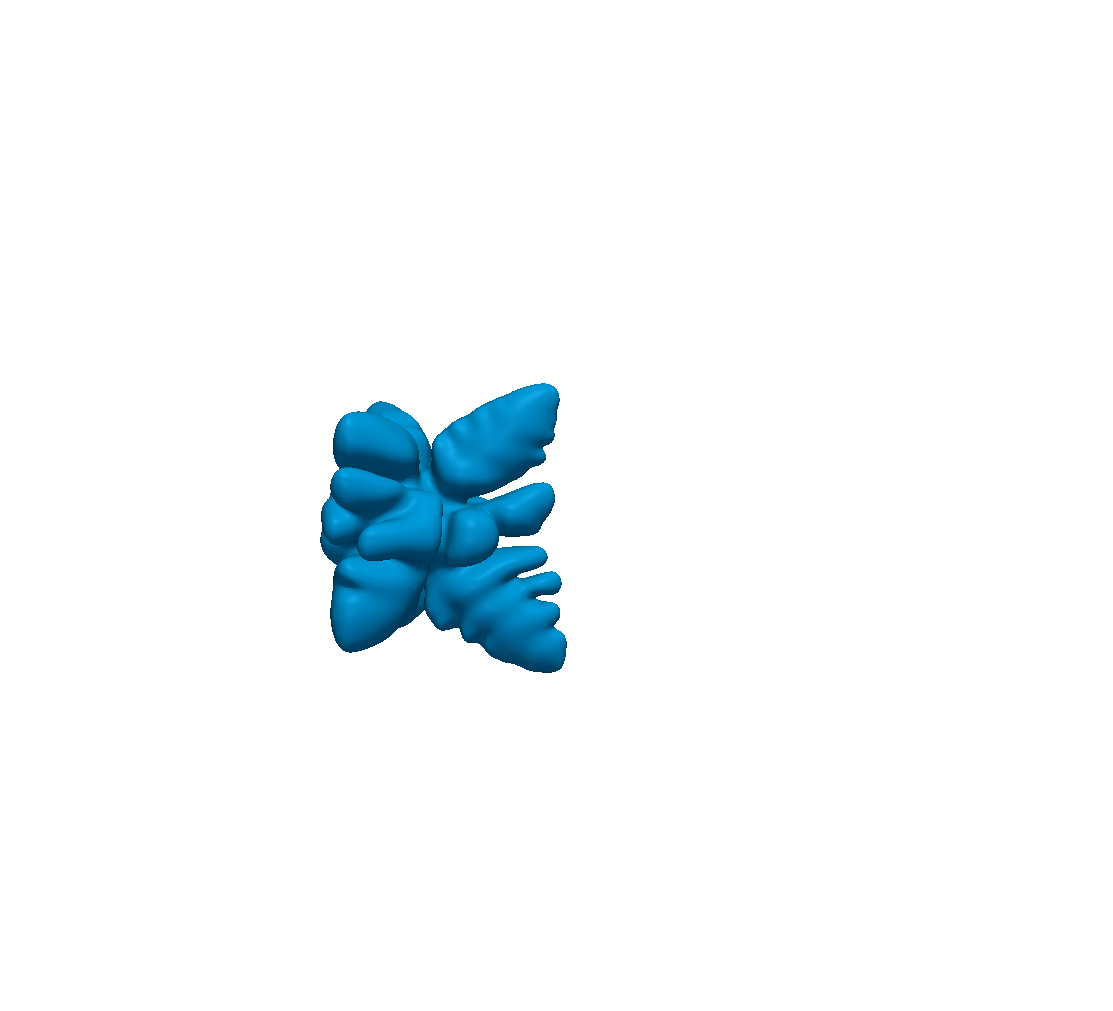
\includegraphics[width=.24\textwidth]{stefan/nb8_iter19.png}
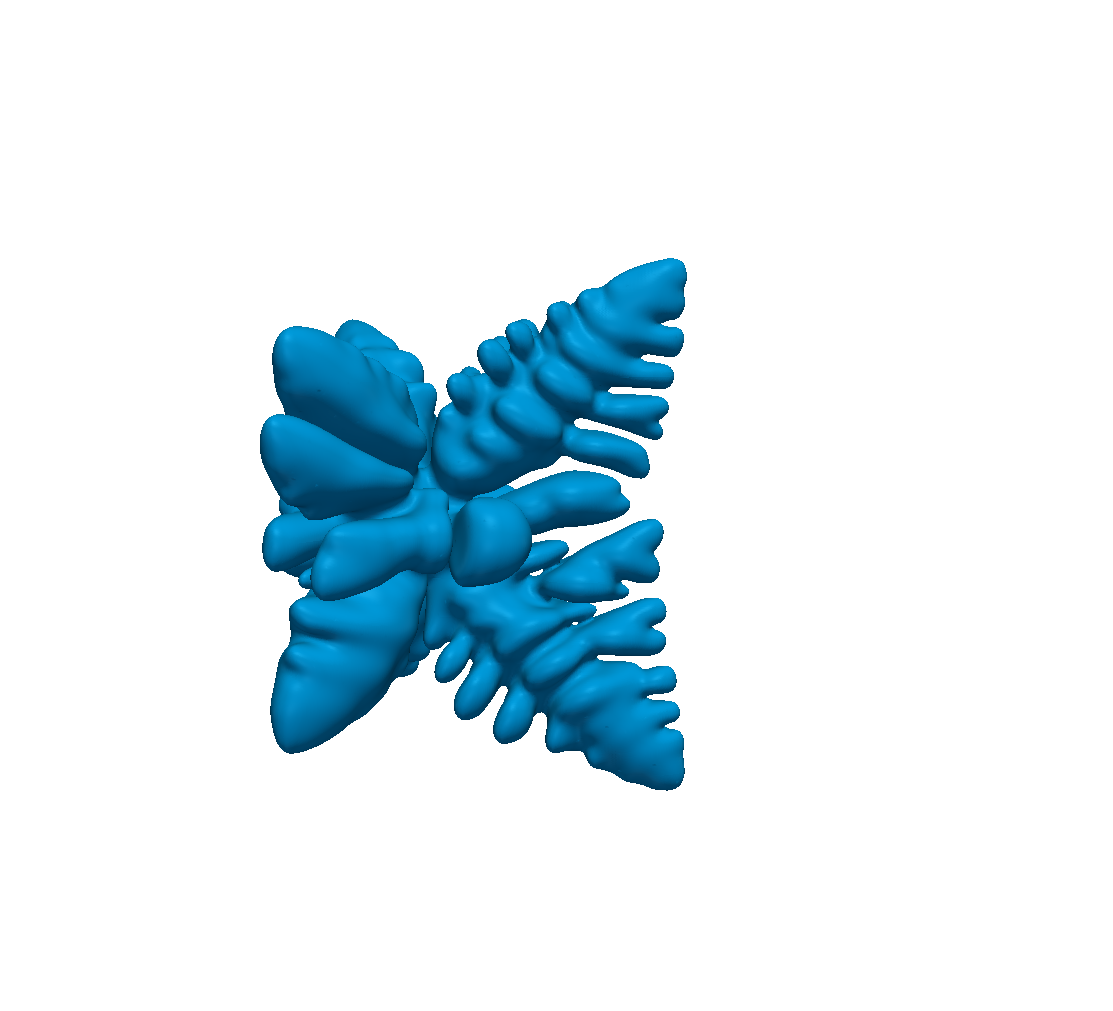
\includegraphics[width=.24\textwidth]{stefan/nb8_iter39.png}
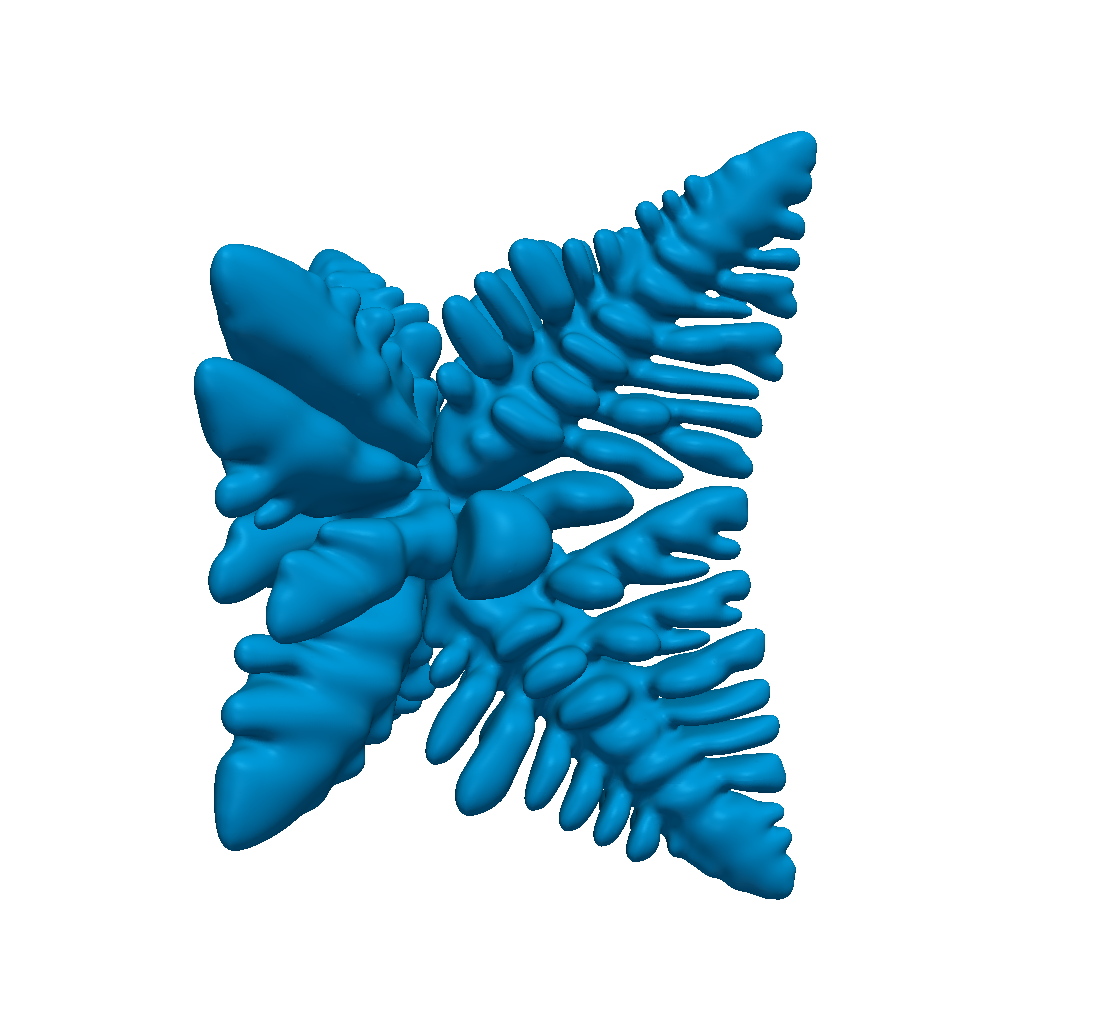
\includegraphics[width=.24\textwidth]{stefan/nb8_iter59.png}
\includegraphics[width=.24\textwidth]{stefan/nb8_iter79.png}
}
\subfigure{
\includegraphics[width=.24\textwidth]{stefan/nb12_iter19.png}
\includegraphics[width=.24\textwidth]{stefan/nb12_iter39.png}
\includegraphics[width=.24\textwidth]{stefan/nb12_iter59.png}
\includegraphics[width=.24\textwidth]{stefan/nb12_iter79.png}
}
\caption{Time evolution of four of the crystals obtained for the Stefan problem simulation. The snapshots represent, from left to right, iterations 96, 196, 296 and 396.} \label{fig:stefan_evolution}
\end{center}
\end{figure}

% %!TEX root = draft.tex
\section{Conclusions}
In this article we have presented parallel algorithms for the advection and reinitialization of the level-set functions on adaptive Quadtree and Octree grids using domain decomposition approach. These algorithms are implemented using a combination of \texttt{MPI} and the open-source \texttt{p4est} library. An important feature of the semi-Lagrangian method is its unconditional stability property which must be preserved in parallel, requiring a parallel interpolation scheme. However, due to the non-uniform distribution of departure points, scalable implementation of such algorithm is not trivial on adaptive Quadtree and Octree grids. An asynchronous interpolation algorithm is presented using non-blocking point-to-point communications which proves good scalability. 

The scalability of the semi-Lagrangian algorithm, however, depends on the CFL number. Great scalability is observed for intermediate CFL numbers while, e.g. $\text{CFL}\sim10$. At higher CFL numbers, however, the departure points are potentially further dispersed across processors which limits the scalability. This is because the domain decomposition technique used here is based on the Z-ordering of cells and does not take the velocity field information into account. A possible remedy for this problem could be assigning weights to cells based on some estimate of what the grid should look like after one step of the advection algorithm, e.g. by using a forward-in-time integration of grid points. Such an estimate could also reduce the number of semi-Lagrangian iterations. These ideas are postponed for further investigations. We have also presented a simple parallelization technique for the reinitialization algorithm based on the pseudo-time transient formulation. Both the semi-Lagrangian and the reinitialization algorithms show good scalability up to 4096 processors. 

Finally, an application of these algorithms is presented in modeling the solidification process by solving a Stefan problem. This application clearly illustrates the applicability of our algorithms to complex multi-scale problems that cannot be treated using the normal domain decomposition techniques on uniform grids. We believe that our findings would be of interest to other researchers who use the level-set framework for similar complex and multi-scale problems.

\section*{Acknowledgment} 
The funding for this project was provided by \mohammad{the funding agency}. We would also like to thank the technical staff at the Texas Advanced Computing Center (TACC) and the developer community of PETSc library for their valuable suggestions during this project.

\bibliographystyle{plain}
\addcontentsline{toc}{section}{\refname}
\bibliography{casl,refs}

\end{document}